\chapter{\gkchapter{Morphèmes et syntaxèmes}{Unités de forme \textit{vs} unités de combinatoire}}\label{sec:2.2}

\section{Principe de commutation}\label{sec:2.2.0}

Le principe de commutation est le principe de base de l’\textstyleTermes{analyse distributionnelle} (voir \sectref{sec:2.1.7} sur \textit{L’identification des unités de la langue}). Il consiste à utiliser la commutation comme mode de décomposition des signes linguistiques.

\Definition{\textstyleTermes{commutation}, \textstyleTermes{environnement}}
{Une \textstyleTermes{commutation} est le remplacement d’un segment de texte par un autre. Par exemple, on peut passer de \textit{construction} à \textit{destruction} en commutant \textit{con-} /\textstylePhono{k\~{ɔ}-}/ avec \textit{de-} /\textstylePhono{de-}/. Une commutation a toujours lieu dans un \textstyleTermes{environnement} donné : ici l’environnement considéré est {\longrule}\textit{struction}.}

La commutation d’un élément permet de dissocier cet élément de son environnement. La commutation précédente permet de postuler la décomposition suivante : \textit{construction} = \textit{con} + \textit{struction}.

\Definition{\textstyleTermes{concaténation}}
{L’opération de combinaison des signifiants la plus élémentaire, consistant à la simple juxtaposition des signifiants l'un à côte de l'autre, est appelée la \textstyleTermes{concaténation}. Pour noter la concaténation, nous utilisons le symbole +, dont nous limiterons ensuite l'usage aux concaténations de segments qui ne sont pas réellement des signes linguistiques.}

Nous nous limitons pour l’instant à la combinaison des signifiants par concaténation (les signifiants sont collés les uns à la suite des autres), mais on verra par la suite qu’il existe des signes qui ont des signifiants discontinus et d’autres dont les signifiants fonctionnent comme des opérateurs (voir l’alternance dans la \sectref{sec:2.2.22} sur \textit{Amalgame, alternance et mégamorphe} et la troncation dans l’\encadref{sec:2.2.25} sur \textit{Syntaxème zéro et troncation en français}).

\section{Commutation et exclusion mutuelle}\label{sec:2.2.1}

Pour considérer qu’il y a vraiment commutation, il faut remplir une condition supplémentaire qu’on appelle l’\textstyleTermes{exclusion mutuelle}. Considérons des énoncés comme \textit{Pierre vient demain} et \textit{Pierre vient en voiture}. On ne veut pas dire ici que \textit{demain} et \textit{en voiture} commutent dans l’environnement «~\textit{Pierre vient {\longrule}}~», car les deux compléments sont cumulables (\textit{Pierre vient en voiture demain}) et qu’aucun n’est obligatoire (\textit{Pierre vient}). Il est donc clair que \textit{demain} et \textit{en voiture} n’occupent pas à proprement parler la même place et ne se remplacent pas l’un l’autre.

\Definition{\textstyleTermes{commutation  (avec exclusion mutuelle)}}
{Nous dirons donc que deux signes A et B \textstyleTermes{commutent} dans l’environnement X{\longrule}Y s’ils \hi{peuvent se remplacer} l’un l’autre et qu’en plus ils \hi{s’excluent} l’un l’autre, c’est-à-dire que XAY et XBY sont acceptables et que XABY et XBAY sont inacceptables.}

Par exemple, A = \textit{pas} et B = \textit{jamais} commutent dans l’environnement \textit{Pierre ne vient {\longrule}} \textit{en voiture}. Ou encore A = \textit{{}-ait} et B = \textit{{}-era} commutent dans l’environnement \textit{chant{\longrule}}.

L’exclusion mutuelle joue un grand rôle théorique, car elle permet de postuler des positions structurales : deux éléments qui s’excluent mutuellement occupent généralement la même \textstyleTermes{position structurale}, puisqu’ils se «~remplacent~» l’un l’autre. Lorsque la structure s’entend en termes de combinaisons libres, nous parlerons de \textstyleTermes{structure syntaxique} et \textstyleTermes{positions syntaxiques} (voir \chapref{sec:3.3}). Lorsque la structure s’entend en termes de précédence et de contiguïté, c’est-à-dire d’ordre linéaire, nous parlerons de \textstyleTermes{structure topologique} et \textstyleTermes{positions topologiques} (voir \chapref{sec:3.5}).

\Definition{\textstyleTermes{paradigme de commutation}}
{Un ensemble de signes qui peuvent commuter les uns avec les autres est appelé un \textstyleTermes{paradigme de commutation}.}

Une position structurale est caractérisée par le paradigme des éléments qui peuvent occuper cette position.

\Definition{\textstyleTermes{paire minimale}}
{Un couple d’exemples qui se caractérise par une commutation minimale est appelé une \textstyleTermes{paire minimale}.}

Par exemple, u = \textit{Pierre ne vient pas en voiture} et v = \textit{Pierre ne vient jamais en voiture} constituent une paire minimale : on passe de u à v par la commutation de \textit{pas} et \textit{jamais} et cette commutation est minimale, car on ne pourrait faire une commutation raisonnable sur un segment plus petit que \textit{pas} ou \textit{jamais}. Le couple \textit{chantait} vs \textit{chantera} n’est pas une paire minimale, car il possible de faire une commutation sur un segment plus petit et de mettre en rapport \textit{chantait} avec \textit{chanterait} et \textit{chanterait} avec \textit{chantera}.

\section{Décomposition propre des signes}\label{sec:2.2.2}

Le fait qu’une commutation soit possible n’assure pas que les unités dégagées soient des signes linguistiques ; il faut pour cela des conditions supplémentaires. Si la commutation entre \textit{con-} et \textit{de-} dans la paire minimale \textit{construction} vs \textit{destruction} est linguistiquement intéressante, c’est parce que \textit{construction} et \textit{destruction} sont deux signes sémantiquement liés et qu’on peut postuler que la commutation de \textit{con-} et \textit{de-} au niveau des signifiants est corrélée au changement de sens au niveau des signifiés. L’existence d’autres paires comme \textit{constitution} et \textit{destitution} et donc d’une décomposition potentielle \textit{con} + \textit{stitution} permet de renforcer le statut de \textit{con-} /\textstylePhono{k\~{ɔ}-}/ comme unité de la langue. Mais pour que \textit{con-} soit réellement considéré comme le signifiant d’un signe, il aurait fallu que sa contribution sémantique soit équivalente dans \textit{construction} et \textit{constitution}, ce qui n’est pas la cas.

Nous allons ajouter une condition qui assure qu’un segment mis à jour par une commutation possède un signifié et définir un \hi{principe de commutation enrichi} qui prend en compte le signe dans sa globalité, signifié et syntactique compris.

\Definition{\textstyleTermes{décomposition propre}}
{Le signe X \textstyleTermes{se décompose proprement} en A + B si X = A + B, s’il existe des segments A’ et B’ tels A + B’, A’ + B et A’ + B’ soient des signes et si {A +} {B est à A’} {+} {B ce que A +} {B’} {est à A’} {+} {B’} (ou, ce qui revient plus ou moins au même, si A~+ B est à A~+ B’ ce que A’ + B est à A’ + B’).}

\Definition{\textstyleTermes{opération de combinaison propre}}
{Nous notons ${\boxplus}$ l’\textstyleTermes{opération de combinaison propre}. La notation «~X = A ${\boxplus}$ B~» signifie donc que X \hi{se décompose proprement} en A et B.}

Quand nous exigeons que A + B soit à A’ + B ce que A + B’ est à A’ + B’, nous mesurons aussi bien la \hi{différence de signifiants} entre A + B et A’ + B que la \hi{différence de syntactiques ou de signifiés}.

Prenons quelques exemples. Le signe X = \textit{un chat} se décompose proprement en A~${\boxplus}$ B avec A = \textit{un} et B = \textit{chat}. On peut en effet faire commuter A avec A’ = \textit{le} et B avec B’ = \textit{chien~}; les quatre combinaisons sont des signes (\textit{un chat, le chat, le chien, un chien}) et \textit{un chat} est à \textit{le chat} ce que \textit{un chien} est à \textit{le chien}. Ou encore \textit{un chat} est à \textit{un chien} ce que \textit{le chat} est à \textit{le chien}.

Le signe X = \textit{avançait} se décompose proprement en A ${\boxplus}$ B avec A = \textit{avanç-} et B~= \textit{{}-ait}. On peut en effet faire commuter A avec A’ = \textit{recul-} et B avec B’ = \textit{{}-era~}; les quatre combinaisons sont des signes (\textit{avançait, avancera, reculait, reculera}) et \textit{avançait} est à \textit{avancera} ce que \textit{reculait} est à \textit{reculera}.

Le signe X = \textit{broyeur} se décompose proprement en A ${\boxplus}$ B avec A = \textit{broy-} et B~=  \textit{{}-eur}. On peut en effet faire commuter A avec A’ = \textit{compress-} et B avec B’ =     \textit{{}-ons~}; les quatre combinaisons sont des signes (\textit{broyeur, broyons, compresseur, compressons}) et \textit{broyeur} est à \textit{broyons} ce que \textit{compresseur} est à \textit{compressons}.

Un cas particulier important est celui où A existe en tant que signe autonome et l’on peut donc prendre pour B’ un segment vide. On a alors :

\Definition{\textstyleTermes{décomposition propre}}
{Le signe X \textstyleTermes{se décompose proprement} en A + B si X = A + B, si A est un signe et s’il existe un autre signe A’ tel que A’ + B soit un signe et que A + B soit à A’ + B ce que A est à A’ (ou, ce qui revient plus ou moins au même, que A~+ B soit à A ce que A’ + B est à A’).}

Ainsi le signe X = \textit{facilement} se décompose proprement en A ${\boxplus}$ B avec A = \textit{facile} et B = \textit{{}-ment}, puisqu’on peut faire commuter A avec A’ = \textit{utile} et que \textit{facilement} est à \textit{facile} ce que \textit{utilement} est à \textit{utile}.

On peut représenter l’application du principe de commutation enrichi par un \textstyleTermes{rectangle analogique}. Les quatre combinaisons A + B, A + B’, A’ + B et A’ + B’ occupent les quatre coins du rectangle et les côtés opposés du rectangle indiquent des rapports de proportionnalité équivalents :

\begin{figure}
\caption{\label{fig:}Rectangle analogique}
\begin{tikzpicture}[baseline]
  \matrix [matrix of nodes, row sep=1cm, column sep=1cm, nodes={font=\strut}] 
    (matrix1) {
    A + B  & A' + B\\
    A + B' & A' + B'\\
    };
  \draw (matrix1-1-1) -- (matrix1-1-2)
                      -- (matrix1-2-2)
                      -- (matrix1-2-1)
                      -- (matrix1-1-1);
  \matrix [right=1cm of matrix1, matrix of nodes, row sep=1cm, column sep=1cm, 
           nodes={font=\strut}] 
    (matrix2) {
    \textit{broy+eur}    & \textit{compress+eur}\\
    \textit{broy+ons}    & \textit{compress+ons}\\
    };
  \draw (matrix2-1-1) -- (matrix2-1-2)
                      -- (matrix2-2-2)
                      -- (matrix2-2-1)
                      -- (matrix2-1-1);
\end{tikzpicture}
\end{figure}


\Definition{\textstyleTermes{diagrammaticité}}
{Un signe linguistique qui se décompose proprement est dit \textstyleTermes{diagrammatique}.}

On peut voir la \textstyleTermes{diagrammaticité} comme la possibilité d’être décomposé par un diagramme tel qu’un rectangle analogique. Un signe diagrammatique est nécessairement construit à partir d’autres signes et sa constructionalité est \hi{visible} (\textstyleTermes{iconique} dirait le logicien américain Charles S. Peirce, qui est à l’origine d’une grande partie de la terminologie utilisée aujourd’hui en sémiotique et notamment du terme \textit{diagramme}).

Lorsqu’un signe X se décompose proprement en A ${\boxplus}$ B, on peut attribuer des sens à A et B de telle façon que le sens de X se calcule de manière \hi{relativement compositionnelle} à partir des sens de A et de B. On en déduit que :

\Definition{\textstyleTermes{signe linguistique}}
{Si le signe X se décompose proprement en A ${\boxplus}$ B, alors A et B peuvent être considérés comme des \textstyleTermes{signes linguistiques}.}

 En effet, comme la commutation est propre, on peut considérer que la contribution de A est la même dans A + B et A~+~B’ et évaluer cette contribution, notamment lorsqu’on connaît déjà le sens de B et B’.

Les \hi{composants} d’une décomposition propre \hi{ne préexistent pas} nécessairement à la décomposition. C’est parce qu’une décomposition potentielle vérifie le principe de commutation enrichi que cette décomposition est propre et que les composants peuvent être reconnus comme des signes. Prenons l’exemple de \textit{broyeur}. Pour l’apprenant du français, le signe -\textit{eur} ne préexiste pas à la décomposition des mots de type \textit{broyeur} et \textit{compresseur}. C’est parce qu’un \textit{broyeur} est à \textit{broyons} ce qu’un \textit{compresseur} est à \textit{compressons} que l’on peut décomposer \textit{broyeur} et donner un sens à \textit{{}-eur} (un X-\textit{eur} est une machine qui sert à X-\textit{er}) et considérer que \textit{broyeur} = \textit{broy}~${\boxplus}$~\textit{eur} (voir discussion dans l’\encadref{sec:2.2.3} sur \textit{La quatrième proportionnelle}).

La conséquence de la remarque précédente est que les signes ne sont pas des éléments donnés a priori, des briques qui préexisteraient à la construction des énoncés. C’est au contraire des énoncés auxquels nous sommes confrontés que nous extrayons ces briques, que nous pouvons ensuite assembler autrement pour construire de nouveaux énoncés.

Attention : \hi{on ne confondra pas la diagrammaticité avec la compositionalité}. Nous donnerons au terme \textit{compositionalité} une acception beaucoup plus restrictive (voir la \sectref{sec:2.3.2} \textit{Chaque sémantème suppose un choix}). La diagrammaticité est une notion un peu floue et graduelle, comme l’est la notion de décomposition propre. Le sens que nous attribuons à un signe comme \textit{{}-eur} est vague. Un compresseur n’est pas n’importe quel appareil qui sert à compresser (un compresseur compresse de l’air et pas autre chose) et c’est en ce sens que la combinaison \textit{compress}~${\boxplus}$~\textit{eur} n’est pas stricto sensu \textit{compositionnelle}. La diagrammaticité est une forme \hi{faible} de la compositionalité.

\loupe[sec:2.2.3]{La quatrième proportionnelle}{%
    L’énonciation du \hi{principe de commutation enrichi} est postérieure aux travaux de Saussure. Mais elle est sous-jacente à la notion fondamentale de \textstyleTermesapprofondissement{rapports associatifs}, que \citet[177, 179]{saussure1916cours} oppose aux \textstyleTermesapprof{rapports syntagmatiques}, et que l’on nomme aujourd’hui, à la suite de Louis \citet{hjelmslev1943omkring} et de Roman \citet{jakobson1959linguistic}, les \textstyleTermesapprofondissement{rapports paradigmatiques~}:

    \begin{quote}
    «~En dehors du discours, les mots offrant quelque chose de commun s’associent dans la mémoire, et il se forme ainsi des groupes au sein desquels règnent des rapports très divers. Ainsi le mot \textit{enseignement} fera surgir inconsciemment devant l’esprit une foule d’autres mots (\textit{enseigner}, \textit{renseigner}, etc., ou bien \textit{armement}, \textit{changement}, etc., ou bien \textit{éducation}, \textit{apprentissage}) ; par un côté ou un autre, tous ont quelque chose de commun entre eux. […]

    Le rapport syntagmatique est \textit{in praesentia~}; il repose sur deux ou plusieurs termes également présents dans une série effective. Au contraire le rapport associatif unit des termes \textit{in absentia} dans une série mnémonique. […]

    Quand quelqu’un dit \textit{marchons} !, il pense inconsciemment à divers groupes d’associations à l’intersection desquels se trouve le syntagme \textit{marchons} ! Celui-ci figure d’une part dans la série \textit{marche} ! \textit{marchez} !, et c’est l’opposition de \textit{marchons} ! avec ces formes qui détermine le choix ; d’autre part, \textit{marchons} ! évoque la série \textit{montons} ! \textit{mangeons} ! etc., au sein de laquelle il est choisi par le même procédé ; dans chaque série, on sait ce qu’il faut faire varier pour obtenir la différenciation propre à l’unité cherchée. »
    \end{quote}

    Bien qu’il n’ait pas explicitement introduit le \textstyleTermesapprofondissement{rectangle analogique} (que certains attribuent au typologue Joseph Greenberg), \citet[228, 231]{saussure1916cours} montre le rôle de la \textstyleTermesapprofondissement{quatrième proportionnelle} dans la construction de nouvelles unités significatives :

    \begin{quote}
    «~ Toute création analogique peut être représentée comme une opération analogue au calcul de la quatrième proportionnelle. […] \textit{Magasinier} n’a pas été engendré par \textit{magasin~}; il a été formé sur le modèle de \textit{prisonnier :} \textit{prison}, etc. […] Pour former \textit{indécorable}, nul besoin d’en extraire les éléments (\textit{in-décor-able}) ; il suffit de prendre l’ensemble et de le placer dans l’équation :
        
        \begin{quote}
        \textit{pardonner :} \textit{impardonnable}, etc., = \textit{décorer : x}.\\
        \noindent\textit{x} = \textit{indécorable}. […]
        \end{quote}

    Sur le modèle de \textit{pension :} \textit{pensionnaire}, \textit{réaction : réactionnaire}, etc., quelqu’un peut créer \textit{interventionnaire} ou \textit{répressionnaire}, signifiant «~qui est pour l’intervention~», «~pour la répression~» :
    
        \begin{quote}
        \textit{réaction :} \textit{réactionnaire} = \textit{répression : x.}\\
        \noindent\textit{x} = \textit{répressionnaire}. […]
        \end{quote}

    À tout instant on rencontre des combinaisons sans lendemain que la langue n’adoptera probablement pas. Le langage des enfants en regorge, parce qu’ils connaissent mal l’usage et n’y sont pas encore asservis ; ils disent \textit{viendre} pour \textit{venir}, \textit{mouru} pour \textit{mort}, etc. Toutes ces innovations sont en soi parfaitement régulières ; elles s’expliquent de la même façon que celles que la langue a acceptées ; ainsi \textit{viendre} repose sur la proportion :

    \begin{quote}
    \textit{éteindrai :} \textit{éteindre} = \textit{viendrai : x}.\\
    \noindent\textit{x} = \textit{viendre}.~»
    \end{quote}
    \end{quote}

    Il est important de noter qu’il y a chez Saussure une très grande réticence à considérer les éléments qui commutent comme des signes : «~Pour former \textit{indécorable}, nul besoin d’en extraire les éléments (\textit{in-décor-able})~». Comme il le montre, il n’est effectivement pas nécessaire d’extraire les composants pour expliquer la formation de nouvelles unités significatives. Aujourd’hui encore une telle décomposition (et la notion de \textit{morphème} qui en découle) est mise en question. La décomposition des signes en signes non autonomisables (c’est-à-dire qui ne peuvent être prononcés seuls et être interprétés seuls) est d’une certaine façon une abstraction, bien utile cependant pour la modélisation des langues. Ce ne sont pas des observables au sens strict, mais des constructions théoriques.
}
\section{Quasi-signes}\label{sec:2.2.4}

Si nous reprenons notre exemple initial, on peut placer les mots \textit{construction,} \textit{destruction, constitution} et \textit{destitution} aux quatre coins d’un rectangle, mais il n’y a pas de rapports de proportionnalité entre les côtés de ce rectangle : \textit{construction} n’est pas à \textit{destruction} ce que \textit{constitution} est à \textit{destitution}. En fait, il ne semble pas qu’il existe de paire qui permette de former un rectangle analogique avec la paire \textit{construction-destruction}, il n’existe pas d’éléments A’ et B’ qui permettent de valider une décomposition propre de \textit{con} + \textit{struction}. La combinaison \textit{con} + \textit{struction} est donc peu diagrammatique. La diagrammaticité est une notion graduelle et on peut dire que la combinaison \textit{con} + \textit{stitution} est encore moins diagrammatrique, car il y a peu de rapport de sens entre \textit{constitution} et les autres mots en -\textit{stitution} (\textit{destitution, institution, restitution, prostitution}). Pour les formes qui interviennent dans une décomposition impropre, comme \textit{struction} ou \textit{stitution}, nous introduisons le terme \textit{quasi-signe}.

\Definition{\textstyleTermes{quasi-signe}}
{Un \textstyleTermes{quasi-signe} est un segment qui apparaît dans un paradigme de commutation, mais pour lequel la commutation n’est pas (suffisamment) propre. Le quasi-signe possède un signifiant clair, délimité par le principe de commutation, mais ne possède pas de signifié à proprement parler.}

Le symbole + de concaténation, lorsqu'il est utilisé en opposition à l’opération ${\boxplus}$, désigne la combinaison impropre entre des quasi-signes.

La décomposition des signes lorsqu’elle est peu diagrammatique est probablement peu visible au locuteur ordinaire, car elle ne joue pas de rôle en synchronie. Elle permet seulement d’avoir des intuitions sur la parenté et l’origine des mots. Par exemple, il est peu visible que \textit{arriver} et \textit{dériver} sont des mots construits avec les éléments \textit{a-, dé-} et \textit{rive}, sur le même schéma que \textit{aborder} ou \textit{atterrir} ou que \textit{déplacer} ou \textit{déterrer}. Le principe de commutation enrichi s’applique mal à nouveau : si on considère A = \textit{a}{}-, A’ = \textit{dé}{}-, B = \textit{riv}(\textit{er}) et B’ = \textit{port}(\textit{er}), et qu’on les combine, on obtient bien quatre signes \textit{arriver, dériver, apporter, déporter}, mais \textit{arriver} n’est pas exactement à \textit{dériver} ce que \textit{apporter} est à \textit{déporter}. Il y a néanmoins entre \textit{arriver} et \textit{apporter} ou entre \textit{dériver} et \textit{déporter} ou encore entre \textit{arriver} et \textit{dériver} des liens sémantiques. Ces liens permettent d’entrevoir derrière les sens réels de \textit{arriver} et \textit{dériver} des lectures «~compositionnelles~» de \textit{a}{}- + \textit{riv}(\textit{er}) ‘s’approcher de la rive’ et de \textit{dé}{}- + \textit{riv}(\textit{er}) ‘s’éloigner de la rive’. Les affixes \textit{a}{}- et \textit{dé}{}- s’utilisent pour qualifier des mouvements dans un sens ou un autre (de même que dans les prépositions \textit{à} et \textit{de} qui sont aussi les marqueurs de tels mouvements : \textit{il part} \textbf{\textit{à}} \textit{la plage, il part} \textbf{\textit{de}} \textit{la plage}). En conclusion, la décomposition de \textit{arriv}(\textit{er}) en \textit{a}{}- + \textit{riv}(\textit{er}) ne donne pas une combinaison propre, mais elle garde une certaine réalité en synchronie par la proximité des formes \textit{a}{}- et \textit{riv}(\textit{er}) avec d’autres formes qui interviennent dans des signes sémantiquement liés.

\section{Combinaison libre}\label{sec:2.2.5}

Nous avons défini le principe de commutation enrichi à partir d’une commutation sur chacune des deux parties de la combinaison A + B (commutation de A’ avec A, commutation de B’ avec B). Bien entendu, plus le paradigme de commutation est important, plus la combinaison est considérée comme régulière. Nous allons maintenant voir à quelle condition une combinaison relève de la syntaxe.

Si l’on considère le mot \textit{blessure}, on voit que \textit{bless}{}- commute proprement avec \textit{brûl-, griff-, piqu-, égratign-, cass-, fêl-,} … et que par ailleurs -\textit{ure} commute proprement avec \textit{{}-ons, -ez, ais, -a,} … et que toutes les combinaisons deux à deux sont valides (\textit{brûlez, griffais, …}).

Venons-en au point qui nous intéresse : la combinaison \textit{bless~}${\boxplus}$\textit{~ure} est pourtant bien différente de la combinaison \textit{bless~}${\boxplus}$\textit{~ons}. Comment caractériser cette différence ?

Les signes qui commutent proprement avec \textit{bless-} dans \textit{blessons} sont les mêmes que ceux qui commutent avec \textit{bless-} dans \textit{blessez} ou \textit{blessais}. Il s’agit d’une classe que l’on va d’ailleurs retrouver dans de nombreux environnements : la classe des verbes. Rien de cela avec \textit{blessure} : les éléments qui commutent avec \textit{bless-} dans \textit{blessure} forment une classe atypique qui contient un certain nombre de verbes, mais aussi des quasi-signes comme \textit{struct-} ou \textit{fract-}. Autrement dit, aucun autre signe n’a la même distribution que \textit{{}-ure}

\Definition{\textstyleTermes{distribution}}
{Nous appelons \textstyleTermes{distribution} d’un signe l’\hi{ensemble des environnements} dans lequel ce signe peut apparaître.}

\Definition{\textstyleTermes{famille d’environnements}}
{Plus généralement, un \hi{ensemble d’environnements} \hi{compatibles} avec un ensemble donné de \hi{signes} est appelée une \textstyleTermes{famille d’environnements}. La distribution d’un signe est donc la famille d’environnements de ce signe.}

La notion de distribution n’est pas univoque : elle dépend de la \hi{taille des environnements} considérés et de la \hi{nature des environnements} considérés. Nous nous intéressons ici à des environnements étroits, de l’ordre du mot. Nous élargirons l’empan de nos environnements dans le \chapfuturef{17} sur les \textit{Catégories microsyntaxiques}. Par ailleurs, nous ne considérons pour l’instant que la dimension linéaire du texte. Nous verrons dans la partie 3 comment définir une structure syntaxique et c’est sur les environnements structurels que nous appliquerons notre analyse distributionnelle du \chapfuturef{17}. Autrement dit, nos environnements seront des portions de la structure et non des segments de texte.

Revenons à la distribution de \textit{{}-ure}. Cette distribution n’est pas déductible simplement des distributions d’autres signes, par exemple par l’intersection ou la réunion de familles d’environnements d’autres signes (voir l’\encadref{sec:2.2.7} sur la \textit{Théorie des ensembles} ; nous pouvons nous contenter pour l’instant d’une compréhension superficielle de ces notions.). Nous dirons que la distribution de  \textit{{}-ure} est \textstyleTermes{irrégulière}.

Dire que la distribution de -\textit{ure} est irrégulière revient à dire que la classe des signes qui peuvent se combiner avec -\textit{ure} est irrégulière.
On peut alors inverser le point de vue et voir -\textit{ure} comme un environnement.

\Definition{\textstyleTermes{classe distributionnelle}}
{Un \hi{ensemble de signes compatibles} avec un ensemble donné d’\hi{environ\-ne\-ments} est appelé une \textstyleTermes{classe distributionnelle}.}

Nous allons maintenant introduire des notions qui seront centrales dans notre définition de la syntaxe et qui nous permettrons de distinguer une combinaison de signes que nous considérons comme syntaxique d'une combinaison qui ne l'est pas, comme \textit{bless~}${\boxplus}$\textit{~ure}.

\Definition{\textstyleTermes{commutation libre}}
{On dit que A \textstyleTermes{commute librement} dans la combinaison propre A~${\boxplus}$~B si la classe des signes qui \hi{commutent proprement} avec A est assez \textbf{régulière} et peut notamment se déduire des classes de signes qui commutent avec A dans d’autres combinaisons.}

Dans l’énoncé \textit{Le chat avançait}, les quatre sous-segments \textit{le, chat, avanç-, -ait} sont des unités syntaxiques. Chaque segment est bien le signifiant d’un signe comme le montre les commutations propres suivantes :

\ea\gllll  \textit{le}   \textit{chat}   \textit{avanç}-   -\textit{ait}\\
 \textit{un}   \textit{chien}   \textit{grogn}-   -\textit{e}\\
 \textit{mon}   \textit{garçon}   \textit{chant}-   -\textit{era}\\
 \textit{ce}   \textit{public}   \textit{march}-   -\textit{a}\\
\z

Ces commutations sont libres, car chaque élément que nous avons introduit possède à peu près la même distribution que ceux avec lesquels il commute. En particulier, toutes les combinaisons qui résultent des commutations considérées sont valides : \textit{le public grogne, ce garçon avancera}, \textit{mon chat chanta,} etc.

\Definition{\textstyleTermes{combinaison libre}}
{On dit que A et B \textstyleTermes{se combinent librement} si A et B \hi{commutent librement} dans la combinaison propre A~${\boxplus}$~B.}

\Definition{\textstyleTermes{opération de combinaison libre}}
{La notation «~X = A~${\oplus}$~B~» signifie que X est le résultat de la combinaison libre de A et B. On appelle cette opération ${\oplus}$ l’\textstyleTermes{opération de combinaison libre}.}

La combinaison \textit{bless~}${\oplus}$\textit{~ons} est libre, tandis que la combinaison \textit{bless~}${\boxplus}$\textit{~ure} est propre, mais \textstyleTermes{liée}.

\Definition{\textstyleTermes{unité syntaxique}}
{Un \hi{signe linguistique} qui \hi{commute librement} avec son environnement est appelé une \textstyleTermes{unité syntaxique}.}

Voir le \chapref{sec:3.1} pour une définition plus précise de l'unité syntaxique.

\loupe[sec:2.2.6]{Liberté de combinaison et opposition parole-langue}{%
    L’opposition entre combinaison libre et liée marque la frontière entre ce que Saussure nomme la langue et la parole. Les \hi{combinaisons libres} font partie de la \textstyleTermesapprofondissement{parole}, c’est-à-dire des productions que chaque locuteur est libre de créer à sa guise. Les \hi{combinaisons liées}, au contraire, font partie de la \textstyleTermesapprofondissement{langue}, c’est-à-dire des connaissances partagées par les locuteurs d’une même langue et qui constituent leur stock lexical. Saussure (\citeyear{saussure1916cours} : 172) ne dit pas autre chose dans l’extrait suivant (même si la notion de combinaison libre et liée n’est pas définie formellement) :

    \begin{quote}
    «~\hi{Le propre de la parole,} \hi{c’est} \hi{la liberté des combinaisons}. [C’est nous qui soulignons]

    On rencontre d’abord un grand nombre d’expressions qui appartiennent à la langue ; ce sont les locutions toutes faites, auxquelles l’usage interdit de rien changer, même si on peut distinguer, à la réflexion, des parties significatives. […]

    Mais ce n’est pas tout ; il faut attribuer à la langue, non à la parole, tous les types de syntagmes construits sur des formes régulières. […] Quand un mot comme \textit{indécorable} surgit dans la parole, il suppose un type déterminé, et celui-ci à son tour n’est possible que par le souvenir d’un nombre suffisant de mots semblables appartenant à la langue (\textit{impardonnable}, \textit{intolérable}, \textit{infatigable}, etc.). Il en est exactement de même des phrases et des groupes de mots établis sur des patrons réguliers ; des combinaisons comme \textit{la terre tourne}, \textit{que vous dit-il} ? etc., répondent à des types généraux, qui ont à leur tour leur support dans la langue sous forme de souvenirs concrets.

    Mais il faut reconnaître que dans le domaine du syntagme, il n’y a pas de limite tranchée entre le fait de langue, marque de l’usage collectif, et le fait de parole, qui dépend de la liberté individuelle. Dans une foule de cas, il est difficile de classer une combinaison d’unités, parce que l’un et l’autre facteurs ont concouru à la produire, et dans des proportions qu’il est impossible de déterminer~»
    \end{quote}
}
\maths[sec:2.2.7]{Théorie des ensembles}{%
    Pour mieux comprendre la suite, il ne sera pas inutile de rappeler les bases de la \textstyleTermesapprof{théorie des ensembles}. Un \textstyleTermesapprof{ensemble} est composé d’objets qui sont appelés ses \textstyleTermesapprof{éléments}. Par exemple, l’alphabet latin moderne est un ensemble comportant 26 éléments, que l’on appelle des lettres.

    La relation qui lie un élément avec l’ensemble qui le contient est appelée la relation d’\textstyleTermesapprof{appartenance} et est notée \textrm{${\in}$}. Par exemple, le lexème \textsc{manger} appartient à l’ensemble V des verbes du français :
    
    \ea
    \textsc{manger} ${\in}$ V.
    \z
    On peut définir un ensemble de deux façons :
    
    \begin{itemize}
    \item  soit en \textstyleTermesapprof{extension}, en donnant la liste de ses éléments entre accolades : \textrm{V}~= \{~\textrm{\textsc{manger,} \textsc{chanter,} \textsc{dormir,} \textsc{lire,}} \textrm{…} \} ;
    \item soit en \textstyleTermesapprof{intension}, par une définition formelle comme une formule ou une opération : par exemple, \textrm{V} est l’ensemble des syntaxèmes qui peuvent se combiner avec les syntaxèmes flexionnels de temps.
    \end{itemize}
    Il existe un unique \textstyleTermesapprof{ensemble vide}, noté \textrm{${\varnothing}$}, qui est donc le seul ensemble sans éléments.

    On définit une relation entre les ensembles appelée l’\textstyleTermesapprof{inclusion} et notée \textrm{${\subseteq}$}. L’ensemble B est dit \hi{inclus} dans l’ensemble A (et on note B~\textrm{${\subseteq}$}~A) si tous les éléments de B sont dans A. On dit encore que B est un \textstyleTermesapprof{sous-ensemble} de A ou une \textstyleTermesapprof{partie} de A.
    
    \begin{figure}[H]
    \begin{floatrow}
    \captionsetup{margin=.05\linewidth}
    \ffigbox{%
      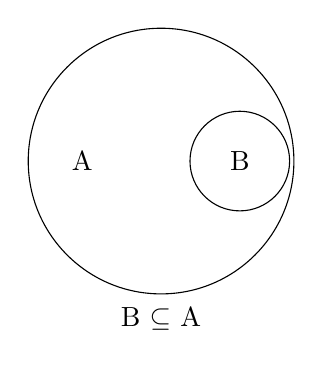
\begin{tikzpicture}
       \node at (0,0) [inner sep=1pt] (A) {A};
       \node at (2,0) (B) {B};
       \draw
          (1,0) circle [draw,radius=48pt] 
          (2,0) circle [draw,clip,radius=18pt];
       \node at (1,-2) {B $\subseteq$ A};
      \end{tikzpicture}}
      {\caption{Inclusion}}
    \ffigbox{%
      \begin{tikzpicture}
       \node at (2,0) (B) {B};
       \filldraw [even odd rule, pattern=north east lines]
          (1,0) circle [draw,radius=48pt] 
          (2,0) circle [draw,clip,radius=18pt];
       \node at (0,0) [inner sep=1pt] (A) {A};
       \node at (1,-2) {$\complement$\textsubscript{A}B}; 
      \end{tikzpicture}}
      {\caption{Complémentaire}}
    \end{floatrow}
    \end{figure}
    
    L’inclusion est une \textstyleTermesapprof{relation d’ordre} (voir la \encadref{sec:3.3.31} \textit{Dépendance, dominance et transitivité} pour une définition formelle) sur les ensembles, similaire à la relation d’ordre ${\leq}$ sur les nombres (d’où la notation \textrm{${\subseteq}$}). Dire «~B \textrm{${\subseteq}$} A~» revient à dire que B est plus petit que A pour la relation d’inclusion. Néanmoins contrairement à la relation ${\leq}$, l’inclusion est un ordre \textstyleTermesapprof{partiel}, puisque deux ensembles peuvent ne pas être ordonnés l’un par rapport à l’autre, notamment lorsqu’ils sont disjoints (c’est-à-dire n’ont pas d’éléments en commun).
                      
    À tout ensemble B inclus dans A, on peut associer le \textstyleTermesapprof{complémentaire} \textrm{${\complement}$}\textsubscript{A}B de B dans A.

    À tout ensemble E, on peut associer l’\textstyleTermesapprof{ensemble des parties} de E, noté 2\textsuperscript{E} ou $\mathcal{P}(\text{E})$, avec un $\mathcal{P}$ comme \textit{partie}. La notation 2\textsuperscript{E} repose sur le fait que si E a \textit{n} éléments, alors 2\textsuperscript{E} a 2\textit{\textsuperscript{n}} éléments.

    Les ensembles \textrm{${\varnothing}$} et E sont respectivement le \textstyleTermesapprof{plus petit} et le \textstyleTermesapprof{plus grand élément} de 2\textsuperscript{E} pour l’inclusion.

    On ne confondra pas l’élément \textit{x} de E avec le \textstyleTermesapprof{singleton} \{~\textit{x}~\}, qui est un élément de 2\textsuperscript{E}.

    On peut définir sur 2\textsuperscript{E} deux opérations binaires, l’union et l’intersection. L’\textstyleTermesapprof{union} de A et B, notée A~\textrm{${\cup}$}~B, est l’ensemble qui contient à la fois les éléments de A et ceux de B, tandis que l’\textstyleTermesapprof{intersection} de A et B, notée A~\textrm{${\cap}$}~B, est l’ensemble des éléments communs à A et B. On peut visualiser ces ensembles sur les schémas suivants :

    \begin{figure}[H]
    \begin{floatrow}
      \captionsetup{margin=.05\linewidth}
      \ffigbox{%
      \begin{tikzpicture}
       \filldraw[pattern=north east lines]
          (0,0) circle [draw,radius=18pt] 
          (1,0) circle [draw,radius=18pt];
       \node at (0,0) [fill=white, circle, inner sep=0pt] (A) {A};
       \node at (1,0) [fill=white, circle, inner sep=0pt] (B) {B};
       \node at (0.5,-1) {A $\cup$ B};
      \end{tikzpicture}}
    {\caption{Union}}                                                                   
    \ffigbox{%
      \begin{tikzpicture}
       \node at (0,0) [inner sep=1pt] (A) {A};
       \node at (1,0) (B) {B};
     \begin{scope}
        \clip (0,0) circle [draw,radius=18pt];
        \fill[pattern=north east lines] (1,0) circle [draw,radius=18pt];
      \end{scope}
       \draw
          (0,0) circle [draw,radius=18pt] 
          (1,0) circle [draw,radius=18pt];
       \node at (0.5,-1) {A $\cap$ B};
      \end{tikzpicture}}
    {\caption{Intersection}}
    \end{floatrow}                                                                 
    \end{figure}

    L’ensemble 2\textsuperscript{E} muni des opérations binaires \textrm{${\cap}$} et \textrm{${\cup}$} et de la relation d’ordre \textrm{${\subseteq}$} possède d’excellentes propriétés similaires à celles de l’ensemble des nombres naturels muni des opérations + et \textrm{${\times}$} et de la relation ${\leq}$. En un sens, ces opérations et relations «~structurent~» l’ensemble 2\textsuperscript{E} ; une telle structure est appelée une \textstyleTermesapprof{structure algébrique}.
    }
\maths[sec:2.2.8]{Dualité}{%
    L’analyse distributionnelle consiste à classer les éléments en fonction de leur distribution dans des combinaisons avec d’autres éléments. La principale difficulté de l’analyse distributionnelle est que tout est interdépendant et que les éléments servent à se classifier les uns les autres. Il existe ainsi une véritable symétrie entre classes distributionnelles et familles d’environnement. Ce type de symétrie est appelé en mathématique la \textstyleTermesapprof{dualité}. Le \textstyleTermesapprof{dual} d’une classe distributionnelle est la famille des environnements compatibles avec les éléments de la classe et le \textstyleTermesapprof{dual} d’une famille d’environnements est la classe distributionnelle des éléments compatibles avec les environnements de la famille. Autrement dit, si A est une classe distributionnelle, \textbf{dual(A)} \textbf{=} \textbf{famille(A)} = “l’ensemble des environnement compatibles avec A” et, si A est une famille d’environnements, \textbf{dual(A)} \textbf{=} \textbf{classe(A)} = “l’ensemble des signes compatibles avec A”.

    Le schéma suivant illustre la dualité. La dualité lie des \textstyleTermesapprof{objets} à des \textstyleTermesapprof{propriétés~}: dans notre cas, les objets sont les signes et les propriétés les environnements (plus exactement la propriété est la compatibilité avec un environnement). Les propriétés définissent des classes d’objets, tandis que les objets définissent des familles de propriétés. Mais le procédé est totalement symétrique et on peut très bien considérer les propriétés comme nos objets et les objets comme leurs propriétés : dans ce cas, les «~propriétés~» d’une propriété donnée sont les objets compatibles avec elle.

    \begin{figure}[H]
    \caption{Dualité entre objets\slash signes et propriétés\slash environnements}
    %% Kudos to Schrödinger's cat for showing the basic workings
    %% of the 3d TikZ library in an unrelated Question at 
    %% https://tex.stackexchange.com/a/548688
    \begin{tikzpicture}[3d view={45}{45},every node/.style={font=\strut}]
      \begin{scope}[canvas is xy plane at z=0,transform shape]
        \draw (0,0) circle [radius=2.5cm] coordinate (circle1);
        \node (classe) [draw,circle] at (-1,0) {classe(A)};
        \node (B) [draw,circle] at (1.5,0) {B};
        \node[left=2.5cm of circle1] {objets};
        \node[right=2.5cm of circle1] {signes};
      \end{scope}
      \begin{scope}[canvas is xy plane at z=-5,transform shape]
        \draw (0,0) circle [radius=2cm] coordinate (circle2);
        \node (A) [draw,circle] at (-1,0) {A};
        \node (famille) [draw,circle] at (.5,0) {famille(B)};
        \node[left=2cm of circle2] {propriétés};
        \node[right=2cm of circle2] {environnements};
      \end{scope}
    \draw  (A.north) -- (classe.335);
    \draw (B) -- (famille.north);
    \end{tikzpicture}
    \end{figure}

    Si A est une classe distributionnelle ou une famille d’environnements, dual(dual(A)) = A. La fonction «~dual~» associe donc une classe à chaque famille, laquelle est elle-même associée à cette classe. On en déduit qu’il y a exactement autant de classes distributionnelles que de familles d’environnements.

    De plus, la fonction «~dual~» possède une excellente propriété qui est de \hi{préserver la structure algébrique} définie par les opérations \textrm{${\cap}$} et \textrm{${\cup}$} et la relation d’ordre \textrm{${\subseteq}$}, puisque dans les deux cas (que A et B soient des classes ou des environnements), on a :

    \begin{enumerate}
    \item  si A~\textrm{${\subseteq}$}~B, alors dual(B)~\textrm{${\subseteq}$}~dual(A) ; autrement dit, plus on considère d’environnements, moins il y a de signes compatibles.
    \item  dual(A~\textrm{${\cup}$}~B) = dual(A)~\textrm{${\cap}$}~dual(B) ; autrement dit, les signes compatibles avec à la fois les environnements dans A et ceux dans B sont, sans surprise, les signes qui sont à la fois compatibles avec A et compatibles avec B.
    \item dual(A~\textrm{${\cap}$}~B) = dual(A)~\textrm{${\cup}$}~dual(B).
    \end{enumerate}

    La dualité inverse les rôles de \textrm{${\cap}$} et \textrm{${\cup}$}, ce qui ne change rien à la structure, car ces deux opérations sont elles-mêmes duales l’une de l’autre. L’ensemble des classes distributionnelles et l’ensemble des familles d'environnements ont donc exactement la même structure algébrique et sont le \hi{miroir l’un} \hi{de l’autre}.
}
\section{Signème}\label{sec:2.2.9}

Nous nous sommes intéressés jusque-là au découpage des signes linguistiques selon l’\textstyleTermes{axe syntagmatique}, c’est-à-dire selon la façon dont ils se combinent ou peuvent être décomposés. Nous allons maintenant nous intéresser à la délimitation des signes selon l’\textstyleTermes{axe paradigmatique} (voir la \sectref{sec:2.1.7} sur \textit{L’identification des unités de la langue} et l’\encadref{sec:2.2.3} sur \textit{La quatrième proportionnelle}). Nous regardons ici le paradigme des environnements pour les différentes occurrences d’une même forme afin de déterminer s’il s’agit des signifiants d’un même signe ou pas.

Considérons par exemple le segment /\textstylePhono{avãs-}/ de \textit{Le chat avançait}. On va retrouver le même segment /\textstylePhono{avãs-}/ dans des énoncés tel que \textit{Nous} \textbf{\textit{avanç}}\textit{ons grâce au vent} et \textit{L’âne ne veut plus} \textbf{\textit{avanc}}\textit{er}. On peut considérer qu’il s’agit du même signe, car sa forme est identique (l’alternance orthographique \textit{c} vs \textit{ç} n’est pas pertinente, la forme orale est identique) et que sa contribution sémantique est identique : ‘avancer’ signifie ici ‘se déplacer vers l’avant’.

Considérons maintenant d’autres occurrences de /\textstylePhono{avãs-}/ dans d’autres environnements :

\begin{figure}
\begin{tikzpicture}
   \matrix (avance) [matrix of nodes,
                     column sep=0pt,
                     every node/.style={inner sep=0pt,font=\strut},
                     column 1/.style={anchor=base east},
                     column 2/.style={nodes={fill=black!15}},
                     column 3/.style={anchor=base west}]
     {
       \textit{Seb a eu de l’}&\textit{avance}&\textit{ment}.\\
       \textit{Bob a fait des}~~&\textit{avance}&\textit{s à Eve}.\\
      \textit{ Zoé a reçu un}e~~&\textit{avance}&~\textit{de 1000 euros}.\\
       \textit{Le chat}~~&\textit{avance}&~\textit{vers moi}.\\
       \textit{Les travaux n’}&\textit{avance}&\textit{nt pas très vite}.\\
       \textit{Ma montre}~~&\textit{avance}&.\\
       \textit{L’}&\textit{avance}&\textit{ment des travaux est moins rapide que prévu}.\\
       \textit{Aya semble}~~&\textit{avance}&\textit{r grâce au vent}.\\
     };
   \draw [-{Triangle[]}] (avance.south west) -- (avance.south east) node [midway,below] {axe syntagmatique};
   \draw [-{Triangle[]}] (avance.south west) -- (avance.north west) node [very near end,left=2ex,rotate=90] {axe paradigmatique};
\end{tikzpicture}
\caption{Découpage de /\textstylePhono{avãs-}/ selon les axes paradigmatique et syntagmatique}
\end{figure}

Dans les énoncés \textit{Ma montre} \textbf{\textit{avanc}}\textit{e} ou \textit{Les travaux n’}\textbf{\textit{avanc}}\textit{ent pas très vite}, nous n’avons plus affaire au même signe /\textstylePhono{avãs-}/, car le sens n’est plus ‘se déplacer vers l’avant’. On peut néanmoins considérer qu’il s’agit, d’un certain point de vue, du même segment, car même si le sens est différent, il reste lié au premier sens que nous avons considéré. Il s’agit d’acceptions métaphoriques : lorsque ma montre avance, c’est comme si l’aiguille avançait plus vite que le temps ; lorsque les travaux avancent, ils se rapprochent de leur achèvement. De plus, la forme du signe est exactement la même et sa combinatoire assez similaire : \textit{avanç-} se combine toujours avec -\textit{ait} (\textit{Ma montre} \textbf{\textit{avanç}}\textit{ait}), mais par contre elle n’accepte plus de complément locatif (\textit{L’âne} \textbf{\textit{avanç}}\textit{ait vers moi ; \textsuperscript{\#}}\textit{Ma montre avance vers moi}). Bien qu’il s’agisse de trois signes différents (puisque les signifiés sont différents), nous considérons pourtant qu’ils appartiennent à une même unité, qu’on nomme généralement le verbe \textsc{avancer}.

On retrouve encore le même segment /\textstylePhono{avãs}/ dans~des énoncés tels que \textit{Pierre est en} \textbf{\textit{avance}}, \textit{Pierre a reçu une} \textbf{\textit{avance}} \textit{de 1000 euros, Pierre a fait des} \textbf{\textit{avance}}\textit{s à Marie}. Ici le sens de /\textstylePhono{avãs}/ est différent, mais surtout sa combinatoire est très différente : ce n’est plus un verbe et il ne peut plus se combiner avec un segment tel que -\textit{ait}. La forme est néanmoins identique et la parenté de sens non négligeable. Dans \textit{L’}\textbf{\textit{avance}}\textit{ment des travaux est moins rapide que prévu} ou \textit{Pierre a eu de l’}\textbf{\textit{avance}}\textit{ment}, /\textstylePhono{avãs}/ est encore un signe (\textit{avancement} est à \textit{avancer} ce que \textit{changement} est à \textit{changer}), mais sa combinatoire est encore différente puisqu’il est indissociable de \textit{{}-ment}.

Tout locuteur du français voit un lien entre toutes les occurrences d’/\textstylePhono{avãs}/ que nous avons considérées. Nous considérons donc que, d’un certain point de vue (et d’un certain point de vue seulement), il s’agit toujours du même objet : un tel objet est appelé un signème.

\Definition{\textstyleTermes{signème}}
{Un \textstyleTermes{signème} est un \hi{ensemble de signes ou de quasi-signes} de \hi{même forme} et de \hi{sens apparentés}. (Nous considérerons des signèmes de signes de formes différentes à la \sectref{sec:2.2.20} sur l’\textit{Allomorphie}.)}

On peut repérer à l’intérieur d’un signème des sous-ensembles de signes qui ont une distribution comparable. À l’intérieur du signème /\textstylePhono{avãs}/, on repère ainsi trois (sous-)signèmes : le verbe \textsc{avancer}, le nom \textsc{avance} et le radical \textit{avance-} de \textsc{avancement}.

\loupe[sec:2.2.10]{Racine et signème}{%
    Jusqu’où pousser la recherche des segments communs ? Il y a dans les mots \textit{commerce} et \textit{marchand} des segments comparables (/m\textrm{ɛ}rs/ pour \textit{commerce} et /m\textrm{a}r\textrm{ʃ}/ pour \textit{marchand}) qui découlent de fait de la même \textstyleTermesapprofondissement{racine} indo-européenne /m\textrm{ɛ}rk/, que l’on retrouve non altérée dans \textit{mercantile} ou \textit{mercato}. Néanmoins, il est probable que les locuteurs ordinaires du français (c’est-à-dire qui ne sont pas entraînés à analyser leur langue) n’auront pas remarqué cela, malgré la forte parenté sémantique de ces mots.

    Qu’est-ce qui distingue racines et morphèmes ?

    Si nous reconnaissons dans \textit{avancement} le même signème /avãs/ que dans \textit{avançons}, c’est parce que \textit{avancement} est à \textit{avançons} ce que \textit{changement} est à \textit{changeons}. Rien de tel pour \textit{commerce} et \textit{marchand} où il n’y a aucune paire analogue. La mise en évidence d’un segment commun ne relève pas de la grammaire du locuteur et de sa connaissance \hi{de} la langue, mais d’une connaissance \hi{sur} la langue. Le \hi{signème} appartient à l’étude \textstyleTermesapprofondissement{synchronique} de la langue, la \hi{racine} à l’étude \textstyleTermesapprofondissement{diachronique} de la langue et à l’\textstyleTermesapprofondissement{étymologie} (l’étude de l’origine des mots). L’opposition entre \textstyleTermesapprofondissement{synchronie} et \textstyleTermesapprofondissement{diachronie} a été posée par Ferdinand de Saussure ; la synchronie considère un \hi{état de langue} à un moment donné, tandis que la diachronie étudie les \hi{variations} (du grec \textit{dia-} ‘à travers’) entre différents état de langue selon l’axe temporel (\textit{chronos}).

    Donnons deux autres exemples : \textit{avance, avant} et \textit{avantage} ont aussi une racine commune, comme le suggère les proximités de forme et de sens, mais on ne peut parler d’un même signème, puisqu’aucun des liens qui unissent ces mots n’a d’analogue en français. \textit{État} et \textit{constater} ont également une racine commune : la parenté de sens apparaît quand on pense à la synonymie entre \textit{constater} et \textit{faire état} et la parenté de forme devient évidente quand on pense qu’un autre sens de \textit{état} se dit en anglais \textit{state} (et que l’on a noté qu’il existe d’autres paires en français où un /s/ s’est effacé : \textit{été-estival, hôpital-hospitalier}).
}
\section{Signèmes minimaux : morphème et syntaxème}\label{sec:2.2.11}

Si nous considérons maintenant le signème /\textstylePhono{avãs}/, nous voyons qu’il n’est possible de décomposer aucun de ses éléments en deux signes linguistiques. On peut éventuellement essayer avec un segment /\textstylePhono{avã}/ que l’on trouve dans \textit{La plage est} \textbf{\textit{avant}} \textit{le village}, mais on ne voit pas comment la composition du sens de cet /\textstylePhono{avã}/ avec un éventuel signe /\textstylePhono{s}/ pourrait donner le signe \textit{avanç-} /\textstylePhono{avãs-}/. Proposer un signe \textstylePhono{/s/} n’aurait de sens qu’au cas où pour un autre signe X au moins, l’ajout d’un \textstylePhono{/s/} créait le sens ‘se déplacer dans la direction X’, c’est à dire si /\textstylePhono{avã}/ et /s/ se combinaient proprement. Le signème /\textstylePhono{avãs}/ est donc indécomposable.

\Definition{\textstyleTermes{morphème}}
{Un \textstyleTermes{morphème} est un signème dont aucun signe n’est décomposable proprement.}

Les morphèmes sont donc les signèmes minimaux du point de vue de l’opération de combinaison propre ${\boxplus}$. Nous pouvons considérer de même les signèmes minimaux du point de vue de la combinaison libre ${\oplus}$, que nous appelons les syntaxèmes.

\Definition{\textstyleTermes{syntaxème}}
{Un \textstyleTermes{syntaxème} est un signème de signes de la même classe distributionnelle dont certains se combinent librement et dont aucun n’est une combinaison libre de signes.}

Les morphèmes sont les \hi{unités minimales de la morphologie} et les syntaxèmes sont les \hi{unités minimales de la syntaxe}. La définition des syntaxèmes sera précisée dans le \chapref{sec:3.1}.

Reprenons l’exemple du signème /\textstylePhono{avãs}/ : il s’agit d’un morphème, puisqu’aucun de ses éléments n’est décomposable proprement. Il contient deux syntaxèmes que sont \textsc{avancer} et \textsc{avance}. Enfin, \textsc{avancement} est un syntaxème, puisqu’aucune de ses acceptions n’est décomposable librement (seul un petit nombre de morphèmes verbaux permettent la combinaison avec \textit{{}-ment}). Il est néanmoins décomposable proprement et contient une occurrence du morphème /\textstylePhono{avãs}/.

\loupe[sec:2.2.12]{Les termes \textit{morphème} et autres \textit{X-èmes}}{%
    La première étude des règles morphologiques d’une langue remonte à 2500 ans au moins. Il s’agit de l’extraordinaire description du sanskrit védique faite par le linguiste indien Pā\textrm{ṇ}ini, qui comprend une description des morphèmes du sanskrit et des règles de combinaison de leurs signifiants. Les termes \textit{morphème} et \textit{phonème} sont introduits dans les années 1880 par le linguiste polonais Baudouin de Courtenay. La définition formelle des morphèmes et le principe de commutation doivent beaucoup aux travaux des distributionnalistes américains sur les langues amérindiennes (voir l’\encadref{sec:2.1.8} sur \textit{Structuralisme et distributionnalisme}).

    Les termes en -\textit{ème} vont foisonner au cours du 20\textsuperscript{e} siècle. Les termes \textit{lexème} et \textit{grammème} sont couramment utilisés pour désigner respectivement les unités du lexique et celles de la grammaire. Nous introduisons \textit{syntaxème} pour désigner les unités minimales de la syntaxe, qu’elles soient lexicales comme le \textit{lexème} ou grammaticales comme le \textit{grammème}. Le terme \textit{syntaxème} (ou la variante \textit{syntactème}) a été utilisé marginalement par quelques auteurs, mais ne s’est jamais imposé, d’autant que c’est le mot qui est généralement considéré comme l’unité minimale de la syntaxe (contrairement au point de vue défendu ici qui considère qu’il s’agit du syntaxème). Le terme \textit{sémantème}, que nous utiliserons pour désigner les unités minimales de la sémantique, est beaucoup plus courant et a été utilisé par Charles Bally ou Igor Mel’čuk pour désigner les sens lexicaux. Nous lui donnons un sens un peu différent en l’utilisant pour désigner des signes (et pas seulement des signifiés) (voir \chapref{sec:2.3} sur \textit{Sémantèmes et syntaxèmes}). Tous les termes que nous venons de mentionner (\textit{morphème, lexème, grammème, syntaxème, sémantème}) désignent, dans l’acception dans laquelle nous les utilisons, des ensembles de signes. Pour finir, nous introduisons le terme \textit{signème} pour désigner tout ensemble de signes d’un de ces types.
}
\section{Lexème, flexion et grammème}\label{sec:2.2.13}

On distingue deux principaux types de syntaxèmes : les syntaxèmes lexicaux ou lexèmes et les syntaxèmes flexionnels ou grammèmes.

\begin{itemize}
\item \textsc{avancer} est un \textstyleTermes{syntaxème lexical} ou \textstyleTermes{lexème~}: il appartient à une classe distributionnelle \textstyleTermes{ouverte} de syntaxèmes, c’est-à-dire qu’il peut commuter avec un très grand nombre de syntaxèmes, potentiellement illimité (cet ensemble est celui des verbes). De plus, ses sens sont assez précis pour être paraphrasés. Par exemple, dans l’énoncé \textit{Le chat avançait}, \textsc{avancer} signifie ‘se déplacer vers l’avant’ et il commute avec sa définition : \textit{Le chat se déplaçait vers l’avant} est une paraphrase de \textit{Le chat avançait}.
\item {}-\textit{ait} est une \textstyleTermes{désinence}. Il s’agit d’une combinaison de plusieurs syntaxèmes, qui comprend notamment la combinaison libre d’un temps (l’imparfait) et d’un accord en nombre et personne. Les syntaxèmes qui composent une désinence s’appellent des \textstyleTermes{syntaxèmes flexionnels} ou \textstyleTermes{grammèmes}. Désinences et syntaxèmes flexionnels appartiennent à des classes distributionnelles \textstyleTermes{fermées} d’éléments, c’est-à-dire qu’ils commutent avec un nombre restreint d’éléments similaires dont on peut faire la liste exhaustive ; il y a par exemple 48 désinences possibles pour un verbe du français : 6 formes pour chacun des 6 «~temps~» simples (présent, imparfait, futur, conditionnel, passé simple, subjonctif), 3 formes pour l'impératif, 4 formes pour chacun des deux participes, auxquelles il faut encore ajouter la forme infinitive (48 = 6${\times}$6 + 3 + 2${\times}$4 + 1). Les grammèmes expriment des significations grammaticales qui ne peuvent être paraphrasées facilement.
\end{itemize}

Lexème verbal et désinence ne peuvent donc pas être utilisés de manière \textstyleTermes{autonome}. Le lexème et sa désinence sont \textstyleTermes{indissociables} l’un de l’autre : une désinence verbale ne s’utilise pas sans une base verbale et un lexème verbal ne s’utilise pas sans désinence. Ils ne sont donc pas \textstyleTermes{autonomisables} (voir la discussion sur autonomisabilité et indissociabilité dans la \sectref{sec:3.2.11} sur l'\textit{Unité syntaxique autonomisable}). Ceci nous amène à la définition du mot, sur laquelle nous reviendrons au \chapfuturef{14} : un \textstyleTermes{mot} est grosso modo un signe linguistique autonomisable minimal, c’est-dire dont les parties sont indissociables et donc non-autonomisables.

Du fait que les lexèmes verbaux ne sont pas autonomisables, il est d’usage de les nommer par l’une de leurs formes fléchies. L’usage en français est d’utiliser la forme infinitive. Cet usage est purement conventionnel (et pédagogiquement assez mauvais, puisque le radical de l’infinitif n’est généralement pas le radical de base ; voir l’\encadref{sec:2.2.23} sur \textit{Syntaxème zéro et troncation en français}) ; par exemple en grammaire latine, il est d’usage de nommer un lexème verbal par la forme de la 1\textsuperscript{ère} personne du singulier du présent (lat. \textsc{amo} ‘j’aime’) et en grammaire arabe par la forme de la 3\textsuperscript{ème} personne du singulier du passé (ar. \textsc{kataba} ‘il a écrit’). Pour éviter toute confusion entre le lexème et la forme infinitive, nous notons le premier en petites majuscules, \textsc{avancer}, et la deuxième en italique, \textit{avancer}. Les syntaxèmes flexionnels sont désignés par des termes métalinguistiques : présent, pluriel, etc. La forme \textit{avancer} est la combinaison de \textsc{avancer} et de l’infinitif :

\ea
\textit{avancer} = \textsc{avancer} ${\oplus}$ infinitif.
\z

\section{Signème libérable, radical, affixe}\label{sec:2.2.14}

Nous allons caractériser les occurrences des morphèmes au sein des lexèmes, c’est-à-dire les \textstyleTermes{morphèmes sous-lexicaux}. Un lexème qui peut être décomposé en plusieurs morphèmes est dit \textstyleTermes{complexe}.

\Definition{\textstyleTermes{libérable}, \textstyleTermes{morphème libérable}, \textstyleTermes{lexical}}
{Un signème est dit \textstyleTermes{libérable} s’il existe des environnements dans lesquels ce signème commute librement. Un \textstyleTermes{morphème libérable} est donc un morphème qui inclut un syntaxème. Lorsque ce syntaxème est lexical, le morphème est dit \textstyleTermes{lexical}.}

Cette propriété est utilisée pour classifier les morphèmes constitutifs d’un lexème complexe. Si l’on considère le syntaxème \textit{brûlure}, qui se décompose en \textit{brûl}${\boxplus}$\textit{ure}, on constate que \textit{brûl-} est libérable, puisqu’il commute librement dans \textit{nous brûlons}, mais \textit{{}-ure} n’est pas libérable, puisqu’il n’existe aucun environnement où -\textit{ure} commute librement.

\Definition{\textstyleTermes{radical}, \textstyleTermes{affixe}, \textstyleTermes{préfixe}, \textstyleTermes{suffixe}}
{Un morphème, lorsqu’il est l’unique morphème lexical d’un lexème, est appelé le \textstyleTermes{radical} du lexème. Un morphème non lexical est appelé un \textstyleTermes{affixe}. Lorsqu’il précède le radical, il s’agit d’un \textstyleTermes{préfixe} et, lorsqu’il le suit, il s'agit d’un \textstyleTermes{suffixe}.}

Il existe également des lexèmes construits uniquement avec des morphèmes non libérables. En français, un certain nombre de lexèmes, appelés composés savants, sont construits avec deux morphèmes lexicaux empruntés au grec ancien (dont certains sont devenus libérables) : \textit{sismo}${\boxplus}$\textit{graphe, sismo}${\boxplus}$\textit{logue, grapho}${\boxplus}$\textit{logue, géo}${\boxplus}$\textit{graphe, géo}${\boxplus}$\textit{thermie, thermo}${\boxplus}$\textit{mètre, métro}${\boxplus}$\textit{nome}, etc. De tels morphèmes, dont le statut est intermédiaire entre affixe et radical, sont appelés des \textstyleTermes{confixes}, car ils doivent être associés par paire pour former un lexème.

Il faut noter que les termes de \textit{libre} et de \textit{libérable} sont définis ici par des critères purement distributionnels et recouvrent donc des notions syntaxiques. Ils ne doivent pas être confondus avec un autre emploi du terme \textit{libre} (angl. \textit{free form}) dû à \citet[§11.5]{bloomfield1933language} qui est proche de ce que nous avons appelé l’autonomisabilité et qui conduit à appeler \textit{forme liée} (angl. \textit{bound form}) tout affixe. Dans notre terminologie, au contraire, les \hi{syntaxèmes flexionnels}, bien qu’étant des affixes, se combinent librement par définition et sont parfaitement \hi{libérables}. Par contre, ils ne sont \hi{pas autonomisables}, puisqu’ils sont indissociables de lexèmes.

Les notions de radical et d’affixe doivent être étendues par analogie. Ainsi, un quasi-morphème comme \textit{struct-}, bien que non libérable, est également considéré comme un élément lexical et comme le radical de \textit{structure} et de \textit{construction}, car il commute avec des morphèmes lexicaux.

A l’inverse, certains préfixes du français présentent un cas limite d’affixe, puisqu’ils appartiennent à des morphèmes prépositionnels comme le \textit{en} de \textit{il} \textbf{\textit{en}}\textit{terre} ou le \textit{sur} de \textit{il} \textbf{\textit{sur}}\textit{estime}. On considère quand même qu’il s’agit d’affixes, car les prépositions simples forment une classe fermée et sont donc moins lexicales que les morphèmes qui ont des emplois en tant que syntaxèmes appartenant à des classes ouvertes. De plus, la classe distributionnelle des préfixes du français contient quand même une bonne proportion de morphèmes non libérables, comme \textit{con-} ou \textit{in-}, et qui commutent avec les autres (\textbf{\textit{com}}\textit{prendre} vs \textbf{\textit{sur}}\textit{prendre}, \textbf{\textit{in}}\textit{estimable} vs \textbf{\textit{sur}}\textit{estimer}).

\section{Dérivation et composition}\label{sec:2.2.15}

La plupart des lexèmes complexes du français sont construits avec un radical et un certain nombre d’affixes. Par exemple, le lexème \textit{détournement} est construit avec le radical \textit{tourn-}, le préfixe \textit{dé-} et le suffixe \textit{{}-ment}. Les lexèmes complexes comportant un unique morphème lexical sont appelés des \textstyleTermes{dérivés morphologiques}. L’opération qui consiste à ajouter un affixe à un lexème pour former un nouveau lexème est appelée la \textstyleTermes{dérivation morphologique}.

Il existe aussi des lexèmes construits avec plusieurs morphèmes lexicaux, comme \textit{soutien-gorge} ou \textit{bonhomme} : de tels syntaxèmes sont appelés des \textstyleTermes{composés morphologiques}. L’opération qui consiste à combiner deux lexèmes pour former un nouveau syntaxème est appelée la \textstyleTermes{composition morphologique}. Un composé peut être la source d’une dérivation comme dans \textit{bonhommie}.

On peut associer à un lexème complexe une structure morphologique en regardant les portions du lexème qui sont libérables. Une \textstyleTermes{unité morphologique} est soit un morphème, soit une portion libérable d’un lexème. Les unités morphologiques de \textit{détournement} sont les morphèmes \textit{dé-, tourn-} et -\textit{ment} et les combinaisons \textit{détourn-} (\textit{il} \textbf{\textit{détourn}}\textit{ait}) et \textit{détournement.} Par contre °\textit{tournement} n’est pas libérable. On en déduit une \textstyleTermes{structure morphologique} que nous pouvons représenter dans ce cas par un parenthésage : \textit{détournement} = (\textit{dé}${\boxplus}$\textit{tourn})${\boxplus}$\textit{ment}. Ceci induit un \textstyleTermes{chemin dérivationnel} menant du radical du lexème au lexème complet par combinaisons successives de morphèmes. Pour \textit{détournement}, le chemin est \textit{tourn}(\textit{er}) → \textit{détourn}(\textit{er}) → \textit{détournement} et pas \textit{tourn}(\textit{er}) → °\textit{tournement} → \textit{détournement}. Cela signifie que, dans la façon dont est perçu le lexème \textit{détournement}, c’est \textit{dé}{}- qui s’affixe d’abord à \textit{tourn}{}-, puis -\textit{ment} au tout.

L’étude des \textstyleTermes{morphèmes sous-lexicaux}, c’est-à-dire des occurrences d’un morphème à l’intérieur d’un lexème, ne relève pas de la syntaxe et est donc hors de la visée de cet ouvrage. Une telle étude concerne la construction des lexèmes, c’est-à-dire la \textstyleTermes{morphologie constructionnelle} et la \textstyleTermes{lexicologie}. Cette notion est néanmoins essentielle à la compréhension de ce que sont les syntaxèmes et de ce qui les différencie des occurrences liées des morphèmes.

\loupe[sec:2.2.17]{«~Syntaxe~» des morphèmes sous-lexicaux}{%
    Lorsqu’on parle de syntaxe, on parle normalement de combinatoire libre (voir la \sectref{sec:3.1.6} sur \textit{Syntaxe et morphologie}) et lorsqu’on parle de combinatoire libre, on parle de combinaisons qui sont faites par le locuteur au moment de la production d’un nouvel énoncé (voir l’\encadref{sec:2.2.6} sur \textit{Liberté de combinaison et opposition parole/langue}). La combinatoire des sous-morphèmes relève au contraire de la structure d’unités déjà construites et stockées dans le lexique mental du locuteur (même s’il existe la possibilité de construire de nouvelles unités lors de la production avec les constructions productives). Il en découle que l’histoire constructionnelle de ces unités se fait sur un temps beaucoup plus long, bien qu’il en reste des traces en synchronie (par la commutation propre avec d’autres morphèmes). On peut alors se poser la question suivante : la structure des combinaisons de sous-morphèmes est-elle ou non de la même nature que celle des syntaxèmes ?

    Nous étudierons en détail la structure des combinaisons syntaxiques dans la partie 3, dont c’est le sujet central. Les outils que nous introduirons peuvent aussi s’appliquer à la description des combinaisons morphologiques. Nous opposerons en particulier deux approches principales de la structure syntaxique, la syntaxe de dépendance et la syntaxe de constituants. La principale différence entre les deux approches repose sur ce qu’elles encodent prioritairement (voir l’\encadref{sec:3.4.16} \textit{Dépendance et constituance se complètent}). Les structures de constituants permettent d’encoder naturellement l’ordre dans lequel les combinaisons ont lieu et c’est ce que nous avons utilisé pour présenter l’analyse de \textit{détournement}, car nous voulions indiquer que lors de l’histoire dérivationnelle de ce mot, \textit{tourn-} s’est d’abord combiné avec \textit{dé-}, puis \textit{{}-ment}. Ils existent des cas où l’histoire dérivationnelle n’est pas aussi claire en synchronie. Tel est le cas par exemple de \textit{châtaigneraie, pommeraie} ou \textit{orangeraie}. Il s’agit a priori du suffixe \textit{{}-aie} qui appliqué à un nom d’arbre désigne un groupe d’arbres, comme dans \textit{chênaie} ‘groupe de chênes’ ou \textit{peupleraie} ‘groupe de peupliers’, avec en plus une alternance -\textit{ier} /je/ → -\textit{er} /ʁ/. On aurait donc \textit{châtaigneraie} = (\textit{châtaigne}\textrm{${\boxplus}$}\textit{ier})\textrm{${\boxplus}$}\textit{aie}. Mais on peut aussi analyser ces dérivations comme le résultat direct de l’application du suffixe \textit{{}-eraie}, lequel suffixe se rencontre dans \textit{chêneraie} ‘groupe de chênes’ (lexème considéré comme fautif mais largement attesté). On peut représenter cette ambiguïté en utilisant une représentation non parenthésée de la dérivation (\textit{châtaigneraie} = \textit{châtaigne}\textrm{${\boxplus}$}\textit{ier}\textrm{${\boxplus}$}\textit{aie}), qui s’apparente alors à une structure de dépendance, puisqu’on n’indique que \textit{{}-ier} se combine aussi bien avec \textit{châtaigne} que \textit{{}-aie} sans spécifier quelle combinaison a lieu en premier.
}
\loupe[sec:2.2.18]{Sémantique des morphèmes sous-lexicaux}{%
    Le fait qu’un affixe soit toujours un morphème non libérable influe sur la nature même de son sens : l’affixe ne peut jamais être «~isolé~» et son sens ne peut pas être saisi de manière autonome. Le sens d’un affixe n’apparaît que dans la \hi{relation entre deux lexèmes} : le sens de -\textit{ure} naît de la relation entre \textsc{blessure} et \textsc{blesser}. Ainsi le sens d’un tel morphème est nécessairement de nature \hi{opératoire} : il n’est exprimable que dans la relation entre deux sens. Le sens de -\textit{ure} est le sens de l’opération qui permet de construire ‘blessure’ à partir de ‘blesser’ et d’autres paires du même type : une X-ure est le résultat obtenu en X-ant quelqu'un ou quelque chose.

    Il existe aussi des morphèmes, comme le -\textit{aume} de \textit{royaume,} qui n’apparaissent que dans un seul lexème dont la diagrammaticité est suffisamment claire pour qu’on attribue un sens au morphème : le fait que le lien sémantique entre \textit{royaume} et \textit{roi} soit assez simple (un royaume est le territoire sous la tutelle d’un roi) et que la paire \textit{roi}{}-\textit{royaume} soit parallèle à d’autres paires comme \textit{prince}{}-\textit{principauté} ou \textit{duc}{}-\textit{duché}, permet de définir facilement le sens (opératoire) de -\textit{aume}. Par contre, \textit{fur}, qui est pourtant un mot, mais qui n’apparaît que dans \textit{au fur et à mesure} n’a plus de sens accessible en français contemporain, car la construction dans laquelle il entre est isolée et qu’il n’y a jamais de commutation possible sur \textit{fur}. De même, beaucoup de locuteurs du français vont utiliser une locution comme \textit{être dans le collimateur} sans avoir aucune idée de ce qu’est un collimateur (voir l'\encadref{sec:3.1.3} sur \textit{Le collimateur et la sellette} pour d’autres exemples).
}
\eiffel[sec:2.2.19]{À la limite entre morphème sous-lexical et syntaxème flexionnel}{%
    La notion de commutation libre est \textstyleTermesapprofondissement{graduelle} et il est parfois difficile pour certains morphèmes de les situer entre morphème sous-lexical et syntaxème (flexionnel). Le cas du morphème -\textit{ment} qui transforme un adjectif en adverbe est un cas intéressant de morphème qui ne commute pas librement, mais s’en approche néanmoins. Dans de nombreux cas, le changement de partie du discours opéré par \textit{{}-ment} ne s’accompagne d’aucun changement de sens, ce qui signifie que la commutation est propre : cf. le passage de \textit{un départ rapide} à \textit{partir rapidement} ou de \textit{une réflexion intense} à \textit{réfléchir intensément}. Mais la dérivation en -\textit{ment} n’est pas systématiquement possible : cf. \textit{une réflexion poussée}/\textit{élaborée} vs *\textit{réfléchir poussément}/\textit{élaborément}, \textit{un départ inattendu} vs *\textit{partir inattendument}. Même des adjectifs très courant comme \textsc{gros} n’ont pas d’adverbe correspondant : \textit{faire une grosse erreur} vs *\textit{se tromper grossement}. Certains adverbes en \textit{{}-ment} sont fort peu diagrammatiques et ne peuvent pas être décomposés proprement, comme \textit{vraiment}, \textit{carrément} ou \textit{vertement}. En conséquence, la classe des éléments qui se combine avec \textit{{}-ment} comporte pas mal d’irrégularités et est par exemple différente de la classe des adjectifs qui se combinent avec \textit{de façon}, puisqu’on a \textit{de façon poussée, élaborée} ou \textit{inattendue} et pas \textit{de façon verte}. On peut également noter quelques irrégularités morphologiques (voir la \sectref{sec:2.2.20} sur l’\textit{Allomorphie}) dans la combinaison de \textit{{}-ment} et d’un adjectif, toutefois la combinaison libre des verbes avec leur flexion comprend davantage encore d’idiosyncrasies, donc les arguments purement morphologiques ne permettent pas de décider s’il s’agit de combinaison libre ou non.

    Un autre cas discutable est le «~genre~» des noms. Le genre des noms ne doit pas être confondu avec le genre des adjectifs. Le genre des adjectifs est un syntaxème flexionnel qui se combine librement avec l’adjectif. Il n’a aucune contribution sémantique et sert seulement à mieux marquer la dépendance entre le nom et l’adjectif qui le qualifie (ce rôle syntaxique constitue la signification du syntaxème flexionnel). Certains noms varient apparemment en genre comme \textit{lion} vs \textit{lionne}, \textit{acteur} vs \textit{actrice} ou \textit{prince} vs \textit{princesse}. Mais dans ce cas, l’opposition est sémantique et marque une opposition de sexe : la lionne est la femelle du lion. Elle peut s’accompagner d’une variation de sens plus importante, puisque par exemple un prince est toujours le fils d’un roi, tandis qu’une princesse peut être la fille d’un roi ou la femme d’un prince. De même, un lion et une lionne possèdent des différences morphologiques suffisamment importantes, comme la crinière, pour qu’il soit bizarre de dire qu’une lionne est un lion femelle. De plus, cette alternance de genre est assez capricieuse avec de nombreux noms dons le genre est fixe (\textit{grenouille, girafe, chacal, moustique,} etc.), même si l’alternance de sexe reste signifiante et plusieurs cas où deux formes sans liens morphologiques existent (\textit{poule} et \textit{coq} ou \textit{jument} et \textit{étalon}). Citons encore les nombreux trous que des néologismes comme \textit{auteure} ou \textit{professeure} peinent encore à combler. Il y a donc toutes les raisons de considérer le /\textstylePhonoApprofondissement{ɛs}/ de /\textstylePhonoApprofondissement{pr\~{ɛ}sɛs}/ \textit{princesse} comme un morphème sous-lexical plutôt qu’un syntaxème flexionnel.
}
\section{Allomorphie}\label{sec:2.2.20}

Nous n’avons jusque-là considéré que des signèmes dont tous les éléments ont le même signifiant. Il y a néanmoins de bonnes raisons d’élargir la notion de signème et d’accepter des alternances de formes. Ainsi là où le verbe \textsc{avancer} présente une seule forme /\textstylePhono{avãs-}/, le verbe \textsc{aller} présente quatre formes : /\textstylePhono{v/-} dans \textit{tu} \textbf{\textit{v}}\textit{as}, /\textstylePhono{al/-} dans \textit{nous} \textbf{\textit{all}}\textit{ons}, /\textstylePhono{i/-} dans \textit{nous} \textbf{\textit{i}}\textit{rons}, /\textstylePhono{aj/-} dans \textit{qu’il} \textbf{\textit{aill}}\textit{e}. On veut pourtant regrouper ces formes parce que \textbf{\textit{all}}\textit{+ons} est à \textit{avanç+ons} ce que \textbf{\textit{i}}\textit{+rons} est à \textit{avance+rons}. Nous dirons que \textit{all-} et \textit{i-} sont des allomorphes.

\Definition{\textstyleTermes{allomorphie}}
{Pour que les signes A\textsubscript{1} et A\textsubscript{2} soient des \textstyleTermes{allomorphes}, il faut que A\textsubscript{1} et A\textsubscript{2} aient des signifiants différents, mais qu’il existe un signe A’ et un certain nombre de signes B et B’ tels que A\textsubscript{1}+B soit à A\textsubscript{2}+B’ ce que A’+B est à A’+B’. (Cette condition est nécessaire, mais pas suffisante, comme nous allons le voir.)}

Cette propriété est bien vérifiée par notre premier exemple : A\textsubscript{1} = \textit{al-}, A\textsubscript{2} = \textit{i-}, A’ = \textit{avanç-}, B = \textit{{}-ons}, B’ = -\textit{rons} et A\textsubscript{1}+B = \textit{allons} est à A\textsubscript{2}+B’ = \textit{irons} ce que A’+B = \textit{avançons} est à A’+B’ = \textit{avancerons}. Deux allomorphes sont donc des signes différents, puisqu’ils ont des signifiants différents, mais ils se comportent ensemble comme s’ils formaient un unique signe, puisqu’ils commutent avec un même signe A’. On traduit cela en demandant qu’ils commutent proprement avec un tel signe dans un certain nombre d’environnements.

La notion d’allomorphie nous permet d’étendre la notion de morphème.

\Definition{\textstyleTermes{morphème polymorphique}}
{Un \textstyleTermes{morphème polymorphique} est la réunion de plusieurs «~morphèmes~» de formes différentes qui sont des allomorphes les uns des autres.}

La première propriété que nous avons donnée pour définir l’allomorphie n’est pas suffisante. Une autre propriété nécessaire pour être des allomorphes est de se ressembler. Il y a en fait deux types de ressemblance possibles et ainsi deux notions d’allomorphie : l’une, syntaxique, est une allomorphie au sein d’un syntaxème, basée sur une similarité de syntactique ; l’autre, morphologique, est une allomorphie au sein d’un morphème, basée sur la similarité des formes.

\Definition{\textstyleTermes{allomorphie syntaxique}}
{Les signes A\textsubscript{1} et A\textsubscript{2} sont des \textstyleTermes{allomorphes (syntaxiques)} si A\textsubscript{1} et A\textsubscript{2} ont des formes différentes, mais des sens identiques et s’il existe un syntaxème A’ dont l’ensemble des contextes possibles réunit les contextes possibles de A\textsubscript{1} et A\textsubscript{2}.}

Le cas de \textsc{aller} vu précédemment illustre l’allomorphie syntaxique. La réunion des paradigmes de flexion des différents allomorphes de \textsc{aller} comprend une quarantaine formes et est équivalente au paradigme de flexion de n’importe quel verbe.

Un autre exemple d’allomorphie syntaxique est l’alternance des formes /ɛ/ vs /j/ pour l’imparfait (\textit{je chant\textbf{ai}s} vs \textit{nous chant\textbf{i}ons}. En effet, ces deux formes ont exactement les mêmes sens et elles possèdent, à elles deux, la même extension que le syntaxème zéro du présent ou que le syntaxème /ʁ/ du futur.

Le deuxième cas d’allormorphie nous concerne moins, car il ne relève pas de la syntaxe.

\Definition{\textstyleTermes{allomorphie morphologique}}
{Les signes A\textsubscript{1} et A\textsubscript{2} sont des \textstyleTermes{allomorphes (morphologiques)} si A\textsubscript{1} et A\textsubscript{2} ont des formes différentes mais similaires, des sens apparentés et s’il existe des signes A’, B et B’ tels que A\textsubscript{1}+B soit à A\textsubscript{2}+B’ ce que A’+B est à A’+B’.}

Dans le cas de l’allomorphie morphologique, il n’y a plus identité de sens et la combinatoire est généralement très différente : il faut donc que A\textsubscript{1} et A\textsubscript{2} possèdent une proximité formelle suffisante pour qu’on considère qu’ils sont parents. Par exemple, \textit{écriv}{}- et \textit{écrit}{}- sont des allomorphes, car \textit{écrit+ure} est à \textit{écriv+ons} ce que \textit{sculpt+ure} est à \textit{sculpt+ons} et /ekʁit/ et /ekʁiv/ sont formellement proches. La différence de forme peut être plus importante si elle se retrouve plusieurs fois : \textit{construct}{}- et \textit{construis}{}- sont des allomorphes, car \textit{construction} est à \textit{construisons} ce que \textit{instruction} est à \textit{instruisons} ou ce que \textit{destruction} est à \textit{détruisons}.

Par contre, même si \textit{coup} est à \textit{frapp+ons} ce que \textit{gifle} est à \textit{gifl+ons}, on ne dira pas que \textit{coup} est un allomorphe de \textit{frapp-}. Il y a là une trop grande distance formelle. On dira plutôt qu'il y a \textstyleTermes{supplétion} et que \textit{coup} est un \textstyleTermes{supplétif} de \textit{frapp-}.

En général, les allomorphes d’un signème sont en \textstyleTermes{distribution complémentaire}, c’est-à-dire que leurs environnements respectifs sont incompatibles (voir la notion de \textit{complémentaire} en \textit{Théorie des ensembles} dans l'\encadref{sec:2.2.7}). Mais il existe aussi des cas d’alternance de forme dans un même environnement. Par exemple le verbe \textsc{balayer} possède deux allomorphes /\textstylePhono{balɛ}/ et /\textstylePhono{balɛj}/ qui peuvent alterner avec certaines flexions : \textit{ils balaient} vs \textit{ils balayent}.

\eiffel[sec:2.2.21]{Alternance vocalique en français : allomorphie ou alternance phonologique ? }{%
    Identifier le nombre d’allomorphes d’un morphème ne va pas nécessairement de soi. Ainsi le verbe \textsc{céder} alterne apparemment deux formes : \textit{céd}{}- [\textstylePhonoApprofondissement{sed}] dans \textit{nous cédons} et \textit{cèd}{}- [\textstylePhonoApprofondissement{sɛd}] dans \textit{il cède}. Si [e] et [\textstylePhonoApprofondissement{ɛ}] peuvent être distinctifs dans les syllabes ouvertes (CV) finales (cf. l’opposition entre \textit{été} /\textstylePhono{ete}/ vs \textit{était} /\textstylePhono{etɛ}/ en français parisien), ils se neutralisent dans les autres positions et forment ce qu’on appelle un archiphonème, que nous noterons /\textstylePhonoApprofondissement{E}/ : en syllabe fermée (CVC), /\textstylePhonoApprofondissement{E}/ est prononcé [\textstylePhonoApprofondissement{ɛ}] et, en syllabe ouverte non finale, il est prononcé /\textstylePhonoApprofondissement{e}/. Ainsi l’alternance relève complètement de la phonologie du français et \textsc{céder} possède donc un unique morphe /\textstylePhonoApprofondissement{cEd}/. La situation est différente pour \textsc{appeler} qui présente une \textstyleTermes{alternance} entre \textit{appell}{}- /\textstylePhonoApprofondissement{apɛl}/ dans \textit{il appelle} et \textit{appel}{}- /\textstylePhonoApprofondissement{apəl}/ dans \textit{nous appelons~}: ici l’alternance n’a plus de motivation phonologique en français contemporain et il y a bien allomorphie. Le fait que la distribution des deux allomorphes de \textsc{appeler} soit identique à celle des deux prononciations de \textsc{céder} laisse supposer que cette allomorphie résulte d’une alternance phonologique aujourd’hui morte, du même type que celle bien vivante de \textsc{céder}. Une allomorphie de même distribution (et de même origine) se trouve avec les verbes \textsc{mourir} ou \textsc{pouvoir} (\textit{il} \textbf{\textit{meur}}\textit{t} vs \textit{nous} \textbf{\textit{mour}}\textit{ons}, \textit{il} \textbf{\textit{peu}}\textit{t} vs \textit{nous} \textbf{\textit{pouv}}\textit{ons}). Nous verrons un autre cas distributionnellemnt similaire à l’allomorphie avec les verbes dit du 2\textsuperscript{ème} groupe (dans l’\encadref{sec:2.2.25} sur \textit{Syntaxème zéro et troncation en français}).
}
\section{Amalgame, alternance, mégamorphe et morphe}\label{sec:2.2.22}

Nous avons fait jusque-là comme si les signifiants se combinaient de manière \textstyleTermes{concaténative}, c’est-à-dire en s’enchaînant les uns à la suite des autres. Il existe certaines situations où il est difficile de trouver la limite entre un lexème et sa désinence. Par exemple, la forme verbale [\textit{nous}] \textit{sommes} entre dans le paradigme des formes du verbe \textsc{être} et se décompose normalement en un morphe du morphème \textsc{être} et une désinence. Les formes en \textit{{}-mes} de la 1\textsuperscript{ère} personne du pluriel ne se rencontrent plus qu’au passé simple (\textit{nous chant}+\textit{â}+\textit{mes}) et de surcroît aucune autre forme de \textsc{être} n’a le radical \textit{som-}. Il s’agit donc, pour \textit{sommes}, d’une forme amalgamée exprimant conjointement le lexème \textsc{être} et sa flexion.

\Definition{\textstyleTermes{amalgame}, \textstyleTermes{mégamorphe fort}, \textstyleTermes{cumulativité}}
{Une combinaison de syntaxèmes dont le signifiant est indécomposable est appelée un \textstyleTermes{amalgame} ou \textstyleTermes{mégamorphe fort}. Les syntaxèmes au sein d’un amalgame sont réalisés de manière \textstyleTermes{cumulative}.}

Même des syntaxèmes normalement réalisés par des mots séparés peuvent s’amalgamer, comme \textit{au} /\textstylePhono{o}/ en distribution complémentaire avec \textit{à la} /\textstylePhono{ala}/. Les désinences, c’est-à-dire les combinaisons de syntaxèmes flexionnels, sont souvent des mégamorphes forts : par exemple, si on considère que l’accord verbal -\textit{ons} /\textstylePhono\~{ɔ}/ combine un accord en personne (1\textsuperscript{ère} personne) et un accord en nombre (pluriel) (voir discussion sur ce point dans la section sur les \textit{Catégories flexionnelles abstraites} dans le \chapfuturef{15}), cette combinaison est un mégamorphe fort.

Un signe tel que \textit{chevaux} \textstylePhono{/ʃəvo/} pose un problème un peu différent. Ici le principe de commutation s’applique à l’ensemble du signe, signifiant compris : \textit{chevaux} est à \textit{cheval} ce que \textit{animaux} est à \textit{animal}. Il n’est néanmoins pas satisfaisant de décomposer \textit{chevaux} en \textit{chev}+\textit{aux}, car les dérivés de \textit{cheval/chevaux} prennent \textit{cheval} comme base : \textit{chevalin}, \textit{chevalier} ou \textit{chevaleresque}. Même chose pour les dérivés d’autres lexèmes en -\textit{al/-aux~}: \textbf{\textit{animal}}\textit{ité,} \textbf{\textit{métall}}\textit{ique}, \textbf{\textit{canal}}\textit{iser}, etc. Il faut donc considérer que le radical du lexème \textsc{cheval} est \textit{cheval} et que le pluriel est réalisé par une \textstyleTermes{alternance} \textstylePhono{/al/} ${\Rightarrow}$ \textstylePhono{/o/}. Le signifiant de cet allomorphe (syntaxique) du pluriel est ainsi traité comme une \hi{opération} qui transforme le segment terminal du radical /al/ en /o/. En conséquence, le signifiant du pluriel ne peut donc pas être séparé du signifiant lexical dans la forme \textstylePhono{/ʃəvo}/ et cette forme est ainsi \textstyleTermes{non segmentable}, bien qu’elle soit obtenue par la \hi{combinaison régulière} du signifiant lexical et d’une alternance.

\Definition{\textstyleTermes{mégamorphe faible}}
{Un signe dont le signifiant est décomposable sans être segmentable est appelé un \textstyleTermes{mégamorphe faible}.}

Nous avons distingué les signèmes indécomposables, que sont morphèmes, des signes non segmentables, que l'on appelle généralement les morphes.

\Definition{\textstyleTermes{morphe}}
{Un signe non segmentable est appelé un \textstyleTermes{morphe}. Un morphe est soit un allomorphe d'un morphème, soit un mégamorphe fort ou faible.}



\loupe[sec:2.2.23]{Flexions irrégulières}{%
    Pourquoi les formes verbales du présent sont plus irrégulières que celle des autres temps ? Pourquoi les participes passés sont plus irréguliers que les participes présents ? Pourquoi les formes des verbes très utilisées comme \textsc{être,} \textsc{avoir} ou \textsc{aller} sont plus irrégulières que les autres ? Parce que les formes les moins courantes sont construites par analogie par les locuteurs et sont donc régulières, alors que les formes très courantes sont apprises dans leur globalité. Dans ces formes qui ne sont plus décomposées (ou plutôt qui ne sont pas composées au moment de leur utilisation), les signifiés des syntaxèmes tendent à se fusionner. Ceci est vrai dans toutes les langues flexionnelles : l’irrégularité la plus grande concerne toujours les mots les plus courants. Diachroniquement, les hausses et baisses de fréquences d’un mot sont souvent suivies d’une acquisition ou d’une perte d’irrégularité. Cette répartition des irrégularités est un argument en faveur de la fréquence d’usage en tant que variable dans la description linguistique.
}

\section{Syntaxème zéro}\label{sec:2.2.24}

Le cas des syntaxèmes zéro est bien illustré avec la conjugaison du français : lorsqu’on considère les quatre formes suivantes du verbe \textsc{avancer} à la 1\textsuperscript{ère} personne du pluriel, [\textit{nous}] \textit{avançons, avanc}\textbf{\textit{er}}\textit{ons, avanc}\textbf{\textit{i}}\textit{ons, avanc}\textbf{\textit{eri}}\textit{ons}, on voit que le morphème d’accord -\textit{ons} est obligatoire et que les morphèmes \mbox{-\textit{er}-} et  \mbox{-\textit{i}-} peuvent s’intercaler et eux seuls. Dans \textit{nous avançons}, l’absence de ces morphèmes indique que le procès exprimé par le verbe \textsc{avancer} a lieu au moment de l’énonciation (pour une description détaillée des syntaxèmes de temps du français on consultera la section sur le \textit{Temps verbal} au \chapfuturef{15}). La forme \textit{avançons} \textbf{s’oppose} aux autres formes — \textit{avancerons, avancions, avancerions} — qui expriment nécessairement le fait que le procès \textbf{n’}a \textbf{pas} lieu au moment de l’énonciation et ont donc un sens incompatible avec celui de \textit{avançons}. L’absence de -\textit{er}{}- et -\textit{i}{}- est donc signifiante.

\Definition{\textstyleTermes{syntaxème zéro}}
{Lorsque l’\hi{absence} d’un syntaxème est \hi{signifiante}, on peut postuler la présence d’un \textstyleTermes{syntaxème zéro}, c’est-à-dire un syntaxème dont la réalisation morphologique est un \hi{segment vide}. Un syntaxème zéro est noté ${\varnothing}$ dans les analyses morphologiques.}

Les syntaxèmes zéro sont des objets abstraits introduits par les linguistes pour modéliser le caractère obligatoire d’un autre syntaxème. C’est parce que le pluriel doit obligatoirement être marqué sur les noms en anglais, la plupart du temps par \textit{{}-s}, et que donc le singulier est marqué par l’absence de ce syntaxème, que l’on peut dire que le singulier des noms en anglais est marqué par un syntaxème zéro. Dans l’exemple suivant, la première ligne donne le mot anglais décomposé au niveau morphologique et la deuxième ligne sa \textstyleTermes{glose}, indiquant les syntaxèmes en jeu :

\ea
\gll {cat-∅}  \hspace{1em}  {cat-s}\\
      {chat-\SG}  {}  {chat-\PL}\\
\z

Les syntaxèmes zéro appartiennent généralement à un \textstyleTermes{paradigme fermé}, condition propice à ce que \hi{l’absence} \hi{soit signifiante}. Ce sont donc essentiellement des \hi{syntaxèmes flexionnels}. (Voir un contre-exemple dans l'exercice 12 en fin de chapitre.)

On peut contraster le cas des syntaxèmes zéro avec celui, plus habituel, illustré par la paire \textit{nous avançons} vs \textit{nous avançons vite}. Ici l’absence de \textit{vite} n’est pas signifiante et le sens ‘nous avançons’ n’est pas incompatible avec le sens ‘nous avançons vite’. Le syntagme \textit{nous avançons} est simplement \hi{moins spécifié} que \textit{nous avançons vite}. Le cas des syntaxèmes zéro est différent : on ne peut pas dire que \textit{nous avançons} est moins spécifié que \textit{nous avancions} ou \textit{nous avancerons}.

Nous ne parlerons pas de \textit{morphème zéro} comme c’est souvent l’usage. Nous allons même plus loin : la notion de \textit{morphème zéro} n’existe pas, car un syntaxème zéro n’a pas de réalisation phonologique et morphologique. C’est justement l’absence de morphème qui est signifiante. Si le syntaxème zéro possède un signifié similaire à ceux des éléments avec lesquels il «~commute~», il ne possède pas de signifiant morphologique. On peut voir le syntaxème zéro comme un demi-signe dont le signifiant serait purement syntaxique, purement combinatoire (voir la \sectref{sec:2.3.17} sur \textit{Syntaxème et faisceau de signes}, où la notion de demi-signe est développée). La notion de zéro est une notion purement syntaxique, qui met généralement en jeu une catégorie flexionnelle, c’est-à-dire un paradigme fermé de signes qui commutent librement.

On fera attention à ne pas confondre \hi{syntaxème zéro} et \hi{syntaxème vide}. Nous utilisons le terme \textit{vide} pour les signes sémantiquement vides, c’est-à-dire qui n’ont pas de contribution sémantique propre, ce qui est la situation inverse de celle des syntaxèmes zéro (voir la \sectref{sec:2.3.3} sur le \textit{Syntaxème vide}). Néanmoins, nous reprenons pour les syntaxèmes zéro la notation traditionnelle ${\varnothing}$. Ce symbole, qui désigne l’ensemble vide en mathématique (voir l’\encadref{sec:2.2.7} sur la \textit{Théorie des ensembles}), exprime bien le fait que la position «~occupée~» par le syntaxème zéro reste vide.

\eiffel[sec:2.2.25]{Syntaxème zéro et troncation en français}{%
    \tcbsubtitle{Accord en genre des adjectifs} 
    L’accord des adjectifs en français~à l’écrit présente un cas de syntaxème zéro. L’adjectif possède quatre formes : \textit{vert, verte, verts, vertes}. On voit, sur ces formes écrites, que les deux segments -\textit{e}{}- et -\textit{s} peuvent s’ajouter au lexème \textit{vert}{}-. Comme le fait d’ajouter ou de ne pas ajouter ces morphèmes est une décision obligatoire, l’absence de ces morphèmes est signifiante. On est donc conduit, pour l’analyse des formes écrites, à introduire deux syntaxèmes zéro et d’avoir ainsi un système avec deux oppositions : \textrm{${\emptyset}$}\textsubscript{1} vs -\textit{e}{}- correspondant à l’opposition masculin vs féminin, \textrm{${\emptyset}$}\textsubscript{2} vs -\textit{s} correspondant à l’opposition singulier vs pluriel.

    L’étude des formes orales des adjectifs présente un paysage un peu plus complexe : en effet, si l’on regarde les formes \textstylePhonoApprofondissement{/vɛʁ/} vs \textstylePhonoApprofondissement{/vɛʁt/} (\textit{vert} vs \textit{verte} à l’écrit), on voit que le féminin fait apparaître le phonème \textstylePhonoApprofondissement{/t/}, lequel segment sonore, dans une application simple et simpliste du principe de commutation, pourrait être considéré comme le signifiant du féminin. De même, les formes \textstylePhonoApprofondissement{/blã/} vs \textstylePhonoApprofondissement{/blãʃ/, /gʁi/} vs \textstylePhonoApprofondissement{/gʁiz/, /gʁo/} vs \textstylePhonoApprofondissement{/gʁos/, /gʁã/} vs \textstylePhonoApprofondissement{/gʁãd/} (\textit{blanc(he), gris(e), gros(se), grand(e)}) devraient nous amener à considérer que le féminin est successivement exprimé par \textstylePhonoApprofondissement{/ʃ/, /z/, /s/, /d/}. Or les mêmes segments apparaissent dans les dérivés \textbf{\textit{blanch}}\textit{eur,} \textbf{\textit{gris}}\textit{aille,} \textbf{\textit{gross}}\textit{eur} ou \textbf{\textit{grand}}\textit{eur} et font donc partie du signifiant du radical qui sert à les former. Il paraît donc plus judicieux de considérer que ces consonnes finales font partie du signifiant du lexème adjectival et que le masculin se réalise par une \textstyleTermesapprofondissement{troncation} de la consonne finale du radical. On peut hésiter à considérer que la troncation fait partie du signifiant du syntaxème masculin ou bien qu’elle résulte d’une propriété du radical. Nous préférons une solution alternative : la chute de la consonne finale du radical peut être vue comme due à l’absence d’un support pour cette consonne, ce qui nous amène à considérer que le masculin est exprimé par un syntaxème zéro et le féminin par quelque chose qui sert de support à la consonne et que l’on peut modéliser par un syntaxème de signifiant  \textstylePhonoApprofondissement{/-ə/} (e muet), modélisation qui est à l’origine de nos conventions orthographiques.



   \tcbsubtitle{Conjugaison des verbes} 
    Un autre cas intéressant de troncation est celui des verbes du 2\textsuperscript{ème} groupe qui alternent deux formes : \textit{sali}{}- dans \textit{il} \textbf{\textit{sali}}\textit{t} et \textit{saliss-} dans \textit{nous} \textbf{\textit{saliss}}\textit{ons}. Les dérivés, comme \textit{salissure} ou \textit{polissage}, sont construits sur la forme longue. La forme courte est utilisée pour trois formes du présent (\textit{je salis, tu salis, il salit}), le participe passé (\textit{sali}), l’infinitif (\textit{salir}), le futur (\textit{nous salirons}) et le conditionnel (\textit{nous salirions}). On peut faire ici la même analyse que pour la flexion de l’adjectif (/\textstylePhonoApprofondissement{vɛʁ/} vs /\textstylePhonoApprofondissement{vɛʁt}/) et considérer que, en l’absence d’une voyelle de soutien, la consonne finale du radical verbal tombe : les flexions singulier du présent et du participe passé ont donc un signifiant zéro, tandis celle de la 3\textsuperscript{ème} personne du pluriel du présent (\textit{ils salissent}) ou celles du subjonctif (\textit{qu’il salisse}) ont un signifiant \textstylePhonoApprofondissement{{}-}/\textstylePhonoApprofondissement{ə}/ qui maintiendra la consonne finale. Futur et conditionnel sont exprimés par un même morphème consonantique, \textstylePhonoApprofondissement{{}-}/\textstylePhonoApprofondissement{ʁ}/\textstylePhonoApprofondissement{{}-} qui ne permet pas non plus à la consonne finale du radical de se maintenir. On en conclut que le verbe \textsc{salir} possède un morphe unique, /\textstylePhonoApprofondissement{sali(s)-}/, dont la consonne finale chute en l’absence d’un voyelle de soutien. Comme le signifiant unique de \textsc{salir} n’est pas complètement prononcé dans la forme infinitive (\textit{salir}), il serait pédagogiquement plus judicieux de présenter les verbes dans une forme où le lexème apparaît dans sa forme complète (par exemple à l’imparfait qui est la forme la plus régulière des verbes français : \textit{il} \textbf{\textit{saliss}}\textit{ait}).

    On retrouve une conjugaison similaire pour des verbes dit du 3\textsuperscript{ème} groupe comme \textsc{écrire} ou \textsc{construire~}: \textit{il} \textbf{\textit{écri}}\textit{t} vs \textit{il} \textbf{\textit{écriv}}\textit{ait}, \textit{il} \textbf{\textit{construi}}\textit{t} vs \textit{il} \textbf{\textit{construis}}\textit{ait}, mais avec des consonnes finales du radical différentes (/\textstylePhonoApprofondissement{v}/ et /\textstylePhonoApprofondissement{z}/ au lieu de /\textstylePhonoApprofondissement{s}/) et une orthographe différente de l’infinitif peu justifiée (\textit{écri}\textbf{\textit{re}} vs \textit{sali}\textbf{\textit{r}}). Ces verbes présentent néanmoins des différences de conjugaison au participe passé (\textit{la lettre est finie~}vs \textit{la lettre est écri}\textbf{\textit{t}}\textit{e}) et au passé simple (\textit{il salit~}vs \textit{il écri}\textbf{\textit{v}}\textit{it}). D’autres verbes du français possèdent également une consonne finale qui chute devant un morphème zéro (\textit{il} \textbf{\textit{vi}}\textit{t} vs \textit{il} \textbf{\textit{viv}}\textit{ait}, \textit{il} \textbf{\textit{par}}\textit{t} vs \textit{il} \textbf{\textit{part}}\textit{ait, il} \textbf{\textit{dor}}\textit{t} vs \textit{il} \textbf{\textit{dorm}}\textit{ait}), mais qui se maintient devant le syntaxème du futur \textstylePhonoApprofondissement{{}-}/\textstylePhonoApprofondissement{ʁ}/\textstylePhonoApprofondissement{{}-} (\textit{vivre}, \textit{nous vivrons}), éventuellement grâce à une voyelle épenthétique (\textit{part}\textbf{\textit{i}}\textit{r}, \textit{nous part}\textbf{\textit{i}}\textit{rons}).
}
\section{Syntaxème et morphologie}\label{sec:2.2.26}

Cet ouvrage s’intéresse peu aux morphèmes, c’est-à-dire aux unités minimales de forme. Nous nous intéressons à la combinatoire des unités et donc aux unités minimales du point de vue de la combinatoire (libre), ce qui nous a amené à introduire la notion de \textit{syntaxème}. Les syntaxèmes tendent à être aussi des unités minimales de forme, notamment les syntaxèmes flexionnels, ce qui entraîne généralement une confusion entre les notions de \textit{morphème} et de \textit{syntaxème}, accentuée par le fait que la troisième composante du signe, le syntactique, n’est généralement pas considérée. Nous nous intéressons à la \textstyleTermes{morphologie}, c’est-à-dire à l’étude de la combinatoire des signifiants, lorsqu’il s’agit de la combinaison de syntaxèmes. Nous avons introduit dans ce chapitre plusieurs notions qui relèvent directement de la morphologie, comme l’amalgame, l’alternance et la troncation. Nous en reparlerons dans l’encadré sur les \textit{Langues isolantes, agglutinantes et flexionnelles} du \chapfuturef{15}.

On notera pour conclure que nous n’avons pas encore parlé de la notion de \textit{mot}. Celle-ci ne sera définie qu’à la section sur le \textit{Mot} du \chapfuturef{14}. L’ensemble de la partie 4 est consacrée à la \textstyleTermes{nanosyntaxe}, c’est-à-dire à l’étude des combinaisons de syntaxèmes particulièrement cohésives, appelée traditionnellement \textit{morphologie flexionnelle}.

\exercices{%\label{sec:2.2.27}
    \exercice{1} 
    \begin{enumerate}[label=\alph*.]
    \item Montrer que la décomposition \textit{nation} + \textit{al} est propre.
    \item Pourquoi la décomposition \textit{idé(e)} + \textit{al} est-elle moins diagrammatique ?
    \end{enumerate}
    
    \exercice{2} 
    \begin{enumerate}[label=\alph*.]
    \item En 2002, Michel Tournier a écrit un livre intitulé «~\textit{Journal extime~}». De quelle façon ce titre joue-t-il sur les morphèmes ? Même question avec «~\textit{Œuvres anthumes~}» d’Alphonse Allais, sous-titre d’un ouvrage de 1893.

    \item Et en utilisant ci-dessus l’expression «~\textit{jouer sur les morphèmes~}», sur quoi joue-t-on ?
    \end{enumerate}

    \exercice{3} Montrer que le suffixe \textit{{}-eur} qui associe à un verbe X un nom désignant celui qui X-e (le marcheur est celui qui marche) n’est pas un syntaxème flexionnel.

    \exercice{4} Quelle est, en français contemporain, la particularité des formes verbales \textit{ci-\textbf{git}}, \textit{j’ai \textbf{ouï} dire, \textbf{oyez} bonnes gens} ?

    \exercice{5} Soit le corpus de swahili suivant. Il s’agit de formes verbales qui forment à elles seules des phrases du swahili. En considérant que ces formes sont des combinaisons libres, déterminer les différent syntaxèmes qui les composent et en déduire un tableau de conjugaison du swahili. Pour extraire chacun des syntaxèmes, on commencera par repérer des paires minimales et les commutations associées.

    \begin{tabbing}
    24\hspace{2\tabcolsep}\=\hspace{2\tabcolsep}\textit{atakusumbua}\hspace{2\tabcolsep}\=\hspace{2\tabcolsep}‘nous l’aimerons’\kill
    1  \> \textit{atanipenda}   \> ‘il m’aimera’\\
    2  \> \textit{atampenda}    \> ‘il l’aimera’\\
    3  \> \textit{atawapenda}   \> ‘il les aimera’\\
    4  \> \textit{nitampenda}   \> ‘je l’aimerai’\\
    5  \> \textit{utanipenda}   \> ‘tu m’aimeras’\\
    6  \> \textit{tutampenda}   \> ‘nous l’aimerons’\\
    7  \> \textit{nitakupenda}  \> ‘je t’aimerai’\\
    8  \> \textit{atanipiga}    \> ‘il me battra’\\
    9  \> \textit{atampiga}     \> ‘il le battra’\\
    10 \> \textit{nitawapenda}  \> ‘je les aimerai’\\
    11 \> \textit{amenipiga}    \> ‘il m’a battu’\\
    12 \> \textit{amempiga}     \> ‘il l’a battu’\\
    13 \> \textit{alikupiga}    \> ‘il te battait’\\
    14 \> \textit{amekupiga}    \> ‘il t’a battu’\\
    15 \> \textit{atakupenda}   \> ‘il t’aimera’\\
    16 \> \textit{atatupenda}   \> ‘il nous aimera’\\
    17 \> \textit{alimpiga}     \> ‘il le battait’\\
    18 \> \textit{utampenda}    \> ‘tu l’aimeras’\\
    19 \> \textit{watampenda}   \> ‘ils l’aimeront’\\
    20 \> \textit{atakupiga}    \> ‘il te battra’\\
    21 \> \textit{ananipiga}    \> ‘il me bat’\\
    22 \> \textit{anampiga}     \> ‘il le bat’\\
    23 \> \textit{unamsumbua}   \> ‘tu l’ennuies’\\
    24 \> \textit{atakusumbua}  \> ‘il t’ennuiera’\\
    25 \> \textit{alinipiga}    \> ‘il me battait’\\
    26 \> \textit{anakupiga}    \> ‘il te bat’\\
    27 \> \textit{tunakulipa}   \> ‘nous te payons’\\
    28 \> \textit{wametulipa}   \> ‘ils nous ont payés’\\
    \end{tabbing}

    \exercice{6} Décomposer le plus long mot du français, \textit{anticonstitutionnellement}, en morphèmes. Indiquer par des parenthésages dans quel ordre ces morphèmes peuvent se combiner. Étudier la diagrammaticité des différentes combinaisons.

    \exercice{7} Montrer que le \textit{{}-ible} de \textit{lisible} est un allomorphe du \textit{{}-able} de \textit{adaptable}.

    \exercice{8} Quel est le signifiant du morphème dérivationnel dans le mot \textit{définition~}? Comparer avec \textit{compression} et \textit{constitution}.

    \exercice{9} Pourquoi peut-on parler d’allomorphie plutôt que de supplétion dans la relation entre les radicaux \textit{exprim}(\textit{er}) et \textit{express}(\textit{ion}) ?

    \exercice{10} Pourquoi considérer-t-on que le présent de l’indicatif est réalisé par un zéro en français ?

    \exercice{11} On s’intéresse aux alternances de radical dans la conjugaison.
    
    \begin{enumerate}[label=\alph*.]
    \item Montrer que chacun des verbes \textsc{aimer}, \textsc{rigoler} et \textsc{pleurer} alterne deux formes orales du radical.
    \item Quelles sont les conditions qui contrôlent la distribution des deux formes des radicaux de ces verbes ? Montrer que ces alternances sont entièrement déterminées par la phonologie du français.
    \item Comparer leur distribution avec celle des formes des verbes \textsc{appeler} et \textsc{mourir}. Pourquoi s’agit-il d’allomorphie dans ce cas ?
    \end{enumerate}
    
     \exercice{12} Que peut-on dire des radicaux du verbe \textsc{avoir} au présent de l'indicatif ? On pourra en particulier comparer ces formes à celles de \textsc{aller} au même temps, ainsi qu'aux formes du futur de n'importe quelle verbe du français.
}
\lecturesadditionnelles{%\label{sec:2.2.28}
    On peut faire remonter l’analyse morphologique aux tout premiers ouvrages en linguistique et les notions de radical et d’affixe sont déjà bien établies dans l’antiquité. L’intérêt pour la morphologie a été renouvelé au 20\textsuperscript{e} siècle par l’étude de nouvelles langues et notamment les langues amérindiennes. Le livre d’Edward \citet{sapir1921language} est probablement l’ouvrage le plus marquant de cette époque.

    La notion unificatrice de \hi{morphème} est introduite dans Bloomfield (1933) au chapitre 10. La morphologie est traitée aux chapitres 14 et 15. On trouvera notamment la description des formes du masculin des adjectifs français par troncation des formes du féminin (\chapfuturef{15}). On pourra également consulter un article de Joseph H. Greenberg de \citeyear{greenberg1954quantitative} qui propose une étude quantitative des constructions morphologiques dans 8 langues différentes et qui présente une définition du morphème et une classification des opérations morphologiques similaire à la nôtre.

    La \textit{morphologie morphématique} a été en partie rejetée au profit d’une \hi{morphologie lexématique} (voir \cite{beard1995lexeme} et \cite{fradin2003nouvelles} pour une défense de la morphologie lexématique et \cite{haspelmath2013understanding} pour une comparaison des deux approches). Si nous avons maintenu la notion de \textit{morphème} dans notre présentation, nous le distinguons du \textit{syntaxème}, dont nous faisons l’unité minimale de combinaison libre. La notion de \textit{syntaxème} étend la notion de \textit{lexème} en évitant d’introduire une frontière entre les unités du lexique et de la grammaire. Comme dans la morphologie lexématique, nous rejetons l’idée de \textit{morphème zéro}, lui substituant la notion de \hi{syntaxème zéro}, c’est-à-dire d’unité syntaxique qui n’a pas de réalisation phonologique et qui donc précisément ne correspond pas à un morphème. On pourra consulter l’ouvrage d'Alain Leméaréchal de \citeyear{lemarechal1997zeros} consacré aux unités de ce type.

    L’opération de \hi{combinaison libre} \textrm{${\oplus}$} est introduite par Igor Mel’čuk qui nomme cette opération l’\textit{union linguistique}. Elle apparaît dans la plupart de ses ouvrages. Néanmoins, il n’en donne pas, à notre connaissance, de définition et la considère plutôt comme une primitive linguistique. Par ailleurs, il ne l’oppose pas, comme nous, à l’opération \textrm{${\boxplus}$} de combinaison propre, elle même opposée à l’opération + de combinaison impropre.

    La notion de \hi{liberté} telle que nous l’avons introduite peut être attribuée à André \citet{martinet1985syntaxe}, qui n’en donne pas de définition satisfaisante à notre avis, mais considère que «~Les deux monèmes /dòn-/ et /-é/ de \textit{donnait} sont des monèmes libres parce que \textit{donnait} ne se comporte exactement, dans ses rapports avec le contexte, comme aucun monème unique de la langue.~» (p. 34) Il n’y a pas néanmoins chez Martinet de distinction entre syntaxème et sémantème : son «~synthème~», dont il dit qu’il «~se comporte vis-à-vis des autres monèmes de la chaîne comme un monème unique~» (p. 37) (ce qui le rapprocherait du syntaxème), doit au final être rapproché de notre sémantème, puisqu’il se présente comme un «~choix unique~» (p. 36) (voir le \chapref{sec:2.3} sur \textit{Sémantèmes et syntaxèmes}).

    Denis \citet{apotheloz2002construction} propose une présentation très claire de la construction des lexèmes du français. L’émergence de l'unité morphologique \textit{{}-eraie} évoquée dans l'\encadref{sec:2.2.17} sur les morphèmes sous-lexicaux y est expliquée. On pourra également consulter le fascicule de Joëlle \citet{gardes-tamine1990grammaire} pour une introduction à la morphologie. Pour une présentation monumentale de la morphologie, on consultera les 5 volumes du \textit{Cours de morphologie générale} d’Igor \citet{melcuk1993cours}. Le volume 4 présente les morphèmes, l’alternance et la distinction entre \hi{mégamorphes forts} et \hi{faibles}. Enfin l'ouvrage de Martin Haspelmath et Andrea D. Sims (\citeyear{haspelmath2013understanding}) est une présentation simple et assez complète de la morphologie. La notion de \textit{morphe} est développée dans \citet{haspelmath2020morph}.

    \FurtherReading{2-2}
}
\corrections{%\label{sec:2.2.29}
    \corrigé{1} 
    \begin{enumerate}[label=\alph*.]
    \item La décomposition est propre, car \textit{national} est à \textit{nation} ce que \textit{régional} est à \textit{région}.
    \item \textit{Idéal} n’est pas à \textit{idée} ce que \textit{national} est à \textit{nation}. On ne voit pas très bien le lien sémantique entre \textit{idée} et \textit{idéal} et ce que pourrait être la contribution de -\textit{al} dans \textit{idéal}.
    \end{enumerate}

    \corrigé{2} 
    \begin{enumerate}[label=\alph*.]
    \item Le mot \textit{extime} a été créé à partir d’\textit{intime} et du couple \textit{intérieur-extérieur} en appliquant la quatrième de proportionnel de Saussure. Une telle création joue sur les morphèmes en imposant une décomposition \textit{in}+\textit{time} et donc une analyse en deux morphèmes de \textit{intime} que les locuteurs ne font normalement pas. Même chose avec \textit{ant\-hume} créé à partir de \textit{posthume} et du couple \textit{antérieur-postérieur}.

    \item Nous jouons avec l’expression «~jouer sur les mots~». Cette expression est une expression figée (voir \sectref{sec:2.3.7} sur \textit{Phrasème}). La commutation de \textit{mots} par \textit{morphèmes} est normalement illégitime et provoque un défigement de l’expression et donc un jeu sur les mots.
    \end{enumerate}

    \corrigé{3} La combinatoire du suffixe \textit{{}-eur} est irrégulière et imprévisible : certains verbes n’ont pas de dérivé en -\textit{eur} (°\textit{aimeur}, °\textit{arriveur}), d’autres ont des dérivés avec des sens très spécifiques (\textit{rongeur} désigne un type d’animal, \textit{descendeur} s’utilise pour un skieur spécialiste de l’épreuve de descente, etc.). À l’inverse un lexème en \textit{{}-eur} comme \textit{auteur} n’est pas dérivé d’un verbe.

    \corrigé{4} Les formes sont figées et il n’y a plus de combinaison libre du lexème verbal et de sa désinence. Nous ne sommes plus capable de conjuguer ces verbes. Quel était l’infinitif de \textit{git} ? (\textit{gésir~}!)

    \corrigé{5} La décomposition en syntaxèmes repose sur l’hypothèse qu’une \hi{différence de forme correspond à une différence de sens} ou de signification (principe de commutation). Par exemple, pour 1 et 2, on suppose que la différence de forme (\textit{{}-ni-} vs \textit{{}-m-}) correspond à la différence de sens entre les énoncés, c’est-à-dire à un indice objet 1\textsuperscript{ère} personne du singulier vs 3\textsuperscript{ème} personne du singulier (il est préférable de parler ici d’indice pronominal plutôt que de pronom ; voir la notion d’indice pronominal dans l’encadré \textit{Pronoms ou syntaxèmes flexionnels ?} du \chapfuturef{14}). De même, pour 8 et 11, la différence de forme \textit{{}-ta-} vs \textit{{}-me-} correspond a priori au passage du futur au passé ou accompli. (La traduction en français est forcément approximative et ne permet de savoir quel est précisément le sens des syntaxèmes. En tout cas, il est clair que parler de passé composé pour 11 n’aurait aucun sens, car si la forme est composée en français, elle ne l’est évidemment pas en swahili.) En continuant à procéder ainsi, on vérifiera que la conjugaison du swahili est extrêmement régulière pour les formes considérées ici. Les formes verbales du swahili se composent ainsi de quatre syntaxèmes : indice sujet \textrm{${\oplus}$} temps \textrm{${\oplus}$} indice objet \textrm{${\oplus}$} radical verbal.

    \corrigé{6} \textit{anticonstitutionnellement} = [\textit{anti} \textrm{${\boxplus}$} ([(\textit{con} + \textit{stitu}) \textrm{${\boxplus}$} \textit{tion}] \textrm{${\boxplus}$} \textit{el})] \textrm{${\boxplus}$} \textit{ment.} La décomposition de \textit{constitu} en \textit{con} + \textit{stitu} est impropre, comme discuté dans la \sectref{sec:2.2.4}.

    \corrigé{7} \textit{lisible} est à \textit{lisons} ce que \textit{adaptable} est à \textit{adaptons}. On en déduit directement que \textit{lisible} = \textit{lis} \textrm{${\boxplus}$} \textit{ible}, \textit{adaptable} = \textit{adapt} \textrm{${\boxplus}$} \textit{able} et \textit{{}-ible} et \textit{{}-able} sont des allomorphes.

    \corrigé{8} Le radical du verbe \textsc{définir} est \textit{définiss-} /definis/, donc le suffixe de \textit{définition} est \textit{{}-ion} /j\~{ɔ}/. Le suffixe est le même dans \textit{compression}. Par contre, le suffixe de \textit{constitution} est \textit{{}-tion} /sj\~{ɔ}/, puisque le radical du verbe \textsc{constituer} est \textit{constitu-}.

    \corrigé{9} Il existe tout une série de verbes en X-\textit{primer} qui ont un nom dérivé en X-\textit{pression} : \textit{comprimer, déprimer, exprimer, opprimer, réprimer, supprimer}. Ceci permet de postuler que le quasi-morphème -\textit{prim-} a un allomorphe \textit{{}-press-}.

    \corrigé{10} Une forme verbale comme \textit{chantons} /\textstylePhonoApprofondissement{ʃãt}\~{ɔ}/ s’oppose à \textit{chantions} /\textstylePhonoApprofondissement{ʃãtj}\~{ɔ}/ ou \textit{chanterons} /\textstylePhonoApprofondissement{ʃãt}ʁ\~{ɔ}/. Nous sommes dans un paradigme fermé de syntaxèmes et l’absence des morphèmes /j/ ou /ʁ/ est signifiante. Le présent de l’indicatif est donc une unité syntaxique sans réalisation phonologique, c’est-à-dire un signe zéro. Dans le mesure où les morphèmes  /j/ ou /ʁ/ ne s'excluent pas mutuellement et peuvent être combinés dans la forme \textit{chanterions} /\textstylePhonoApprofondissement{ʃãt}ʁj\~{ɔ}/, on peut faire l'hypothèse qu'ils appartiennent à deux paradigmes différents et s'opposent chacun à un syntaxème zéro, dont le présent de l'indicatif serait la combinaison (voir discussion au \chapfuturef{15}).

    \corrigé{11} Tous ces verbes ont une alternance vocalique : \textit{j’aime} [ʒ\textbf{ɛ}m] vs \textit{nous aimons} [nuz\textbf{e}m\~{ɔ}] (voir aussi \textit{je cède} [ʒǝs\textbf{ɛ}d] vs \textit{nous cédons} [nus\textbf{e}d\~{ɔ}]), \textit{je rigole} [ʒǝʁig\textbf{ɔ}l] vs \textit{nous rigolons} [nuʁig\textbf{o}l\~{ɔ}], \textit{je pleure} [ʒǝpl\textbf{œ}ʁ] vs \textit{nous pleurons} [nupl\textbf{ø}ʁ\~{ɔ}], \textit{j’appelle} [ʒap\textbf{ɛ}l] vs \textit{nous appelons} [nuzap\textbf{ǝ}l\~{ɔ}], \textit{je meurs} [ʒǝm\textbf{œ}ʁ] vs \textit{nous mourons} [num\textbf{u}ʁ\~{ɔ}]. Ces alternances ont la même distribution : un radical est utilisé devant un zéro et l’autre devant une voyelle. Pour les trois premiers verbes, il s’agit d’une alternance phonologiquement contrôlée entre [ɛ] vs [e], [ɔ] vs [o] et [œ] vs [ø] selon que le phonème (ou l’archiphonème) est dans une syllabe fermée (CVC) ou ouverte (CV) (voir l’\encadref{sec:2.2.21} \textit{Alternance vocalique en français : allomorphie ou alternance phonologique} ?). Pour les deux derniers verbes, l’alternance a certainement une origine phonologique, mais elle est aujourd’hui réalisée par deux phonèmes bien distincts ([ɛ] vs [ǝ] et [œ] vs [u]) et il s’agit donc d’allomorphie.
    
     \corrigé{12} Les formes du verbe \textsc{avoir} au présent de l'indicatif sont \textit{ai} /ɛ/,  \textit{as} /a/, \textit{a} /a/, \textit{avons} /av\~{ɔ}/, \textit{avez} /ave/, \textit{ont} /\~{ɔ}/. L'alignement avec les formes de \textsc{aller} (\textit{vais} /vɛ/, \textit{vas} /a/, \textit{va} /a/, \textit{allons} /al\~{ɔ}/, \textit{allez} /ale/, \textit{vont} /v\~{ɔ}/) permet de décomposer ces formes et de postuler pour \textsc{avoir} un radical zéro et un radical /av/, pour \textsc{aller} les radicaux /v/ et /al/ et pour les accords les morphes /ɛ/, /a/, /a/, /\~{ɔ}/, /e/ et /\~{ɔ}/, également présents au futur. Cette décomposition est évidemment discutable, car les morphèmes d'accord au présent de l'indicatif ont des formes différentes pour le reste des verbes du français. Si l'on accepte cette décomposition, \textsc{avoir} est un exemple de \hi{lexème zéro}.
}
